\documentclass[11pt,bibtotoc,liststotoc,DIV12,BCOR8,openany,a4paper]{book}

% use this declaration to set specific page margins
%\usepackage[a4paper , lmargin = {2.7cm} , rmargin = {2.9cm} , tmargin = {2.7cm} , bmargin = {4.6cm} ]{geometry}
\usepackage[a4paper]{geometry}

\usepackage[english]{babel}
\usepackage{bibgerm}       		% german references
\usepackage[utf8x]{inputenc} % german characters
\usepackage{graphicx} 				% it's recommended to use PDF images but you can use JPG or PNG as well
\usepackage{url}           		% format URLs
\usepackage{hyperref} 				% create hyperlinks
\usepackage{listings}	% for source code
\lstset{frameround=fttt,language=Python,numbers=left,breaklines=true}
\usepackage{subfig}						% two figures next to each other (example: figure 3a), figure 3b)
\usepackage{scrpage2}					% header and footer line
\setlength{\headheight}{1.1\baselineskip} 

% header and footer line - no header & footer line on pages where a new chapter starts
\pagestyle{scrheadings}
%\ohead{Automatic Service Generation}
\ohead{\headmark}
\automark{chapter}
\ihead{}
% \ihead{\headmark}
% \automark{section}
\cfoot[]{\thepage}
%\ifoot{Future Smart Cam, TU Berlin, Fachgebiet AV, 2009}

% set path where images are stored
\graphicspath{{./img/}}

%
% der Befehl \hypenation versteht keine Sonderzeichen, also weder �
% noch "a noch \"a. W�rter die derartige Zeichen enthalten m�ssen
% direkt im Text getrennt werden, z.B. W�r\-ter
%
\hyphenation{te-le-com-muni-cation 
te-le-com-muni-cation-specific 
Te-le-kom-mu-ni-ka-tions-API
Kon-fi-gu-ra-tions-werk-zeug} 					% use this file to set explicit hyphenations (doesn't seem to work correctly)

%% Useful packages
\usepackage{geometry}
\usepackage{diagbox}
\usepackage{amsmath}
\usepackage{graphicx}
\usepackage[colorinlistoftodos]{todonotes}
%\usepackage[colorlinks=true, allcolors=blue]{hyperref}
\usepackage{url}
\usepackage{minted}
\usepackage{enumitem}
\usepackage{hyperref}
\usepackage{color}
\usepackage{multirow}
\usepackage{longtable}
\usepackage{eurosym}
\usepackage[]{acronym}
\usepackage{setspace}
\definecolor{mypink1}{rgb}{0.858, 0.188, 0.478}

%morpholical box
\usepackage{booktabs}
\usepackage{tikz}
\usetikzlibrary{matrix}

\newcommand{\zeilenabstand}{\normalbaselineskip}

\newcommand\grafik[2]{%
  \begin{minipage}{0.1cm}
    \centering\smash{\raisebox{\tabcolsep}{#1}}%
    \includegraphics[width=\linewidth]{#2}%
  \end{minipage}%
}

\tikzset{vp/.style={circle,fill,inner sep=3pt}}
\newcommand\verbindungslinie[3]{
  \foreach [remember=\p as \lastp (initially #2)] \p in {#3}
    \draw[#1](\lastp.center)node[vp]{}--(\p.center)node[vp]{};
}
%end morphological box

% proto files. See https://github.com/aytchell/latex-listings-protobuf
\newcommand{\SetProtoColorsBlueish}{
  % Colors inspired by the NASM style of Robin Eklind
  % https://github.com/mewspring/latex
  \definecolor{proto_basic}{RGB}{0,0,0}             % black
  \definecolor{proto_keyword}{RGB}{0,0,255}         % blue
  \definecolor{proto_type}{RGB}{128,0,0}            % dark red
  \definecolor{proto_options}{RGB}{128,0,128}       % purple
  \definecolor{proto_comment}{RGB}{0,128,0}         % dark green
  \definecolor{proto_string}{RGB}{255,0,0}          % red
  \definecolor{proto_number}{RGB}{108,113,196}      % violet
  \definecolor{proto_ident}{RGB}{0,0,0}             % black
  \definecolor{proto_digits}{RGB}{0,0,128}          % dark blue
  \definecolor{proto_background}{RGB}{255,255,255}  % white
}

\lstdefinelanguage[2]{protobuf}{%
    sensitive=true,%
    morecomment=[l]{//},%
    morecomment=[s]{/*}{*/},%
    morestring=[b]{"},%
    % For the keywords of Protocol Buffers
    % see https://developers.google.com/protocol-buffers/docs/proto
    morekeywords={enum,oneof,map,syntax,public,import,option,package,message,%
        group,optional,required,repeated,default,reserved,extend,extensions,%
        to,max,service,rpc,returns,true,false},%
    % Basic types
    % see https://developers.google.com/protocol-buffers/docs/proto#scalar
    morekeywords=[2]{%
        double,float,int32,int64,uint32,uint64,sint32,sint64,%
        fixed32,fixed64,sfixed32,sfixed64,bool,string,bytes},%
    % Options
    % taken from 'google/protobuf/descriptor.proto'
    morekeywords=[3]{%
        % Generic Options
        deprecated, uninterpreted_option,%
        % File Options
        java_package,java_outer_classname,java_multiple_files,%
        java_generate_equals_and_hash,java_string_check_utf8,optimize_for,%
        go_package,cc_generic_services,java_generic_services,%
        py_generic_services,cc_enable_arenas,obj_class_prefix,%
        csharp_namespace,%
        % Message Options
        message_set_wire_format,no_standard_descriptor_accessor,map_entry,%
        % Field Options
        ctype, packed,jstype,lazy,weak,%
        % Enum Options
        allow_alias}%
}
\lstalias[]{protobuf2}[2]{protobuf}

\lstdefinelanguage[3]{protobuf}[2]{protobuf}{%
    % Language keywords
    % see https://developers.google.com/protocol-buffers/docs/proto3
    deletekeywords={
        % 'group' was marked as deprecated in protobuf2; now it's disallowed
        group,%
        % in protobuf3 the Any type replaces extensions (from protobuf2)
        extensions, to, extend, max,%
        % 'required' is no longer allowed
        required,%
        % 'optional' is default; stating it explicitly is disallowed
        optional,%
        % explicit default values are no longer allowed
        default}%
}
\lstalias[]{protobuf3}[3]{protobuf}


\lstdefinestyle{protobuf}{
  frame=lines,
  xleftmargin=\parindent,
  belowcaptionskip=1\baselineskip,
  backgroundcolor=\color{proto_background},
  basicstyle=\color{proto_basic}\footnotesize\ttfamily,
	keywordstyle=[1]\color{proto_keyword},
	keywordstyle=[2]\color{proto_type},
	keywordstyle=[3]\color{proto_options},
	commentstyle=\color{proto_comment},
	stringstyle=\color{proto_string},
  numberstyle=\color{proto_number}\tiny,
  identifierstyle=\color{proto_ident},
	numbers=left,
	numbersep=5pt,
	breaklines=true,
	showstringspaces=false,
	tabsize=2,
  % This 'literate' block is responsible for colouring numbers
  % appearing in the code
  literate={0}{{\textcolor{proto_digits}{0}}}{1}%
           {1}{{\textcolor{proto_digits}{1}}}{1}%
           {2}{{\textcolor{proto_digits}{2}}}{1}%
           {3}{{\textcolor{proto_digits}{3}}}{1}%
           {4}{{\textcolor{proto_digits}{4}}}{1}%
           {5}{{\textcolor{proto_digits}{5}}}{1}%
           {6}{{\textcolor{proto_digits}{6}}}{1}%
           {7}{{\textcolor{proto_digits}{7}}}{1}%
           {8}{{\textcolor{proto_digits}{8}}}{1}%
           {9}{{\textcolor{proto_digits}{9}}}{1}%
           {.0}{{\textcolor{proto_digits}{.0}}}{2}%
           {.1}{{\textcolor{proto_digits}{.1}}}{2}%
           {.2}{{\textcolor{proto_digits}{.2}}}{2}%
           {.3}{{\textcolor{proto_digits}{.3}}}{2}%
           {.4}{{\textcolor{proto_digits}{.4}}}{2}%
           {.5}{{\textcolor{proto_digits}{.5}}}{2}%
           {.6}{{\textcolor{proto_digits}{.6}}}{2}%
           {.7}{{\textcolor{proto_digits}{.7}}}{2}%
           {.8}{{\textcolor{proto_digits}{.8}}}{2}%
           {.9}{{\textcolor{proto_digits}{.9}}}{2}%
           % We need to add some hacks - otherwise 'listings' would
           % colour (only) the digits in the types instead of the type
           {int32}{{\textcolor{proto_type}{int32}}}{5}%
           {int64}{{\textcolor{proto_type}{int64}}}{5}%
           {uint32}{{\textcolor{proto_type}{uint32}}}{6}%
           {uint64}{{\textcolor{proto_type}{uint64}}}{6}%
           {sint32}{{\textcolor{proto_type}{sint32}}}{6}%
           {sint64}{{\textcolor{proto_type}{sint64}}}{6}%
           {fixed32}{{\textcolor{proto_type}{fixed32}}}{7}%
           {fixed64}{{\textcolor{proto_type}{fixed64}}}{7}%
           {sfixed32}{{\textcolor{proto_type}{sfixed32}}}{8}%
           {sfixed64}{{\textcolor{proto_type}{sfixed64}}}{8}%
           {java_string_check_utf8}{{%
             \textcolor{proto_options}{java_string_check_utf8}}}{2}%
           {\ }{{ }}{1},
	prebreak=\raisebox{0ex}[0ex][0ex]{\ensuremath{\hookleftarrow}},
	upquote=true,
}
\SetProtoColorsBlueish{}
%end proto files

\onehalfspacing
\Huge
\begin{document}
% ---------------------------------------------------------------
\frontmatter
    \thispagestyle{empty}
\newgeometry{left=2.5cm,right=2.5cm}
\begin{center}

\vspace*{1.4cm}
{\LARGE Technical University of Berlin}

\vspace{0.5cm}
{\large Faculty V - Mechanical Engineering and Transport Systems\\[1mm]}
{\large Department of Machine Tools and Factory Management\\[1mm]}
{\large Divison of Industrial Automation\\[5mm]}

Pascalstr. 8-9\\
10587 Berlin\\
https://www.iat.tu-berlin.de\\

\vspace*{1cm}


\includegraphics[width=3.5cm]{tu_logo.jpg}

\vspace*{1.0cm}

{\LARGE Master's Thesis}\\

\vspace{1.0cm}
{\LARGE \textbf{Automatic Generation of Object Detection Services with Varying Detection Methods and Interfaces}}\\
%\vspace*{0.3cm}

{\LARGE \textbf{}}\\
\vspace*{0.5cm}
{\LARGE Nikolas Keuck}\\
388015\\
nikolas.keuck@gmail.com\\
Major: Computational Engineering Sciences
\\
\vspace*{0.5cm}
Aug 22nd, 2019\\ % 	date of submission
\vspace*{0.5cm}

Referee: Prof. Dr.-Ing. Jörg Krüger\\
Tutor: Dipl.-Ing. Martin Rudorfer

%\vspace{2cm}


\end{center}
\restoregeometry

   	\thispagestyle{empty}
    \cleardoublepage
    
    % \thispagestyle{empty}
\vspace*{1.0cm}

\begin{center}
    {\LARGE \textbf{Acknowledgments}}
\end{center}

\vspace*{0.5cm}

First of all, I would like to thank my supervisor Martin Rudorfer for his constant flow of helpful ideas, high responsiveness and willingness to take time to support me.. It sums up to 15 hours of face to face meetings, 1.5 hours of video calls, 42 e-mails and unknown time for proofreading.\\ \\
\noindent
To my colleagues, namely Wilma, Marian and Nils: Thank you for being so cooperative. You made working full time and writing a master's thesis possible!\\ \\
\noindent
Last but not least, I would like to thank my family and friends who accompanied me over the years of my studies:\\ \\

\textbf{Thank you!}
    % \thispagestyle{empty}
    % \cleardoublepage
    
    % \newpage

\thispagestyle{empty}

\begin{large}

\vspace*{6cm}

\noindent
Hereby I declare that I wrote this thesis myself with the help of no more than the mentioned literature and auxiliary means.
\vspace{2cm}

\noindent
Berlin, August 22nd, 2019

\vspace{3cm}

\hspace*{7cm}%
\dotfill\\
\hspace*{8.5cm}%
\textit{(Signature)}

\end{large}
 
    % \thispagestyle{empty}
    % \cleardoublepage
    
    
    % \thispagestyle{empty}
\vspace*{1.0cm}

\begin{center}
    \textbf{Abstract}
\end{center}

\vspace*{0.5cm}

\noindent
Contemporary manufacturing relies on monolithic object detection (OD) software architecture to achieve high-performance automation. As production machines typically have a life span of over 20 years, object detection aligns to this rigid pattern. Typically, necessary OD hardware is delivered along with the software. In the last decade, OD research leaped forward while product life cycles shortened concurrently. Thus, it is desirable to get more frequent updates. Subsequently, the goals of this thesis are eliminating hardware and saving maintenance costs while simultaneously keeping up to date with state of the art OD methods. This thesis introduces \textit{Recipe Generator}, a framework based on service-oriented architectures. It trains OD services stored in a Docker hub using a computer-aided design file. Then, it combines pairs of trained OD services and camera image acquisition services to recipes. Recipes are transferred, prepared and executed via an open platform communication unified architecture (OPC UA) vision server for easy manufacturing integration. The services are dockerized and communicate via Google remote procedure calls or representational state transfer. The main advantages of this approach are the flexible reuse of existing OD methods and the ease to add new ones in a preferred language and platform. There are two main challenges. The first is to increase the performance, reliability and availability of the framework by, e.g., time-sensitive networking. The second is to enhance the framework with a catalogue for "plug-and-play" services.
    % \thispagestyle{empty}
    % \cleardoublepage
    % % \thispagestyle{empty}
\vspace*{1.0cm}

\begin{center}
    \textbf{Zusammenfassung}
\end{center}

\vspace*{0.5cm}

\noindent

Die moderne Fertigung setzt auf monolithische Softwarearchitekturen in der  Objekterkennung (OE), um eine leistungsstarke Automatisierung zu erreichen. Da Produktionsmaschinen in der Regel eine Lebensdauer von über 20 Jahren haben, richtet sich die Objekterkennung nach diesem starren Muster. In der Regel wird die erforderliche OE-Hardware zusammen mit der Software geliefert. In den letzten zehn Jahren hat die OE-Forschung einen Sprung nach vorne gemacht, während sich gleichzeitig die Produktlebenszyklen verkürzt haben. Daher ist es wünschenswert, häufigere Aktualisierungen zu erhalten. Ziel dieser Arbeit ist es, Hardware zu eliminieren, Wartungskosten zu senken und gleichzeitig auf dem neuesten Stand der OE-Methoden zu bleiben. Diese Arbeit stellt \textit{Recepy Generator} vor, eine Rahmenstruktur (Framework), das auf Dienste-orientierten Architekturen basiert. Es trainiert OE-Services, die in einem Docker-Hub gespeichert sind, mit einer computergestützten Designdatei (CAD). Anschließend werden Paare von trainierten OE-Diensten und Bilderfassungsdiensten zu Rezepten kombiniert. Die Rezepte werden über einen OPC UA Vision-Server in die Fertigung übertragen und dort vorbereitet und ausgeführt. Die Dienste sind dockerisiert und kommunizieren über Googles Fernprozeduraufrufe (gRPC) oder REST. Die Hauptvorteile dieses Ansatzes sind die flexible Wiederverwendung vorhandener OE-Methoden und das einfache Hinzufügen neuer Methoden in einer bevorzugten Sprache und Plattform. Es gibt zwei Hauptherausforderungen. Die erste besteht darin, die Leistung, Zuverlässigkeit und Verfügbarkeit des Frameworks durch z.B. zeitsensitive Vernetzung (TSN) zu erhöhen. Die zweite besteht darin, das Framework mit einem Katalog für sofort betriebsbereite Dienste zu erweitern.
    % % \thispagestyle{empty}
    
    \setcounter{tocdepth}{3}
    \tableofcontents
    \thispagestyle{empty}
    
    \chapter*{List of Acronyms}
\thispagestyle{empty}
\begin{tabbing}
spacespacespace \= space \kill
API	 \> 	Application Programming Interface	 \\
ATAM	 \> 	Architecture Tradeoff Analysis Method	 \\
CAD	 \> 	Computer Aided Design	 \\
CAP	 \> 	Consistency, Availability, Partition Tolerance	 \\
CORBA	 \> 	Common Object Request Broker Architecture 	 \\
CPU	 \> 	Central Processing Unit	 \\
CRUD	 \> 	Create, Retrieve, Update, Delete	 \\
DCOM	 \> 	Distributed Component Object Model	 \\
EMVA \> European Machine Vision Association\\
ESB	\>	Enterprise Service Bus \\
GCV	\>	Google Cloud Vision \\
GraphQL     \>  Graph Query Language\\
gRPC     \>  Google Remote Procedure Call\\
GUI	\>	Graphical User Interface \\
HTTP	 \> 	Hypertext Transfer Protocol	 \\
ISO    \>  International Organization for Standardization\\
IT  \>  Information Technology\\
JSON	\>	JavaScript Object Notation \\
M2M	\>	Machine to Machine \\
MQTT     \>  Message Queuing Telemetry Transport\\
MT      \> Messaging Technology\\
OD     \>  Object Detection\\
ODS     \>  Object Detection Service\\
ODM     \>  Object Detection Method\\
OPC UA     \>  Open Platform Communication Unified Architecture\\
OPC UA VC    \>  Open Platform Communication Unified Architecture Vision Client\\
OPC UA VS    \>  Open Platform Communication Unified Architecture Vision Server\\
OSI     \>  Open Systems Interconnection\\
OT  \> Operation Technology\\
PLC  \> Programmable Logic Controller\\
RAM    \> Read Access Memory \\
REST    \> Representational State Transfer \\
RG    \> Recipe Generator \\
RGB    \> Red Green Blue - Depth \\
RPC    \> Remote Procedure Call \\
SOAP	 \> 	Simple Object Access Protocol	 \\
TCP	 \> 	Transmission Control Protocol	 \\
TSN	 \> 	Time Sensitive Networking	 \\
URL	 \> 	Uniform Resource Locator	 \\
UUID	 \> 	Universally Unique Identifier	 \\
VDMA \>     Verband Deutscher Maschinen- und Anlagenbau (Unternehmen) \\
VM	 \> 	Virtual Machine	 \\
VS  \>  Vision System\\
XML  \>  Extended Markup Language\\
\end{tabbing}
\thispagestyle{empty}
\endinput

    \thispagestyle{empty}
    
    \listoffigures
    \thispagestyle{empty}
    
    \listoftables
    \thispagestyle{empty}
    
    
% --------------------------------------------------------------

\mainmatter % comment single chapters for faster compilation
\parskip=2ex\relax
    \chapter{Introduction\label{cha:chapter1}}
There is a vast variety of different object detection algorithms reaching from feature-based to template-based methods, and more recently, also deep-learning-based approaches. Especially the latter have conquered the field very rapidly and have consistently improved the state of the art in many established object detection benchmarks. However, this improvement has not yet arrived at the shop floors of the manufacturing companies. This is in part due to characteristics of the method, such as the large amount of required training data. However, another reason is that the current machine vision infrastructure is not flexible enough to keep track of the dynamic development in the field of object detection. Deploying or even only trying out a new method typically requires a certain investment in cost and time that has to be justified very well. This workflow can be greatly accelerated by using \textit{Service-Oriented Architectures} (SOA).

The goal of this thesis is to simplify the process of programming an object detector and integrating it into the manufacturing process. In fact, the great aim is to not program anything at all – instead, a framework shall be proposed that allows generating an object detection service from a single example image.
The service should detect the object with a specified method and should automatically have the appropriate interfaces for convenient integration into SOA. The key advantage is that new methods can be tested and deployed without any effort, as we can generate and deploy a service which has the same interface as our old one but an updated method.


 
 TODO: Die Einleitung muss ein wenig ausführlicher sein. Gönn dir ruhig jeweils einen Abschnitt zu: Kontext, konkrete Problemstellung (inkl. der wissenschaftlichen Herausforderungen), und Herangehensweise in deiner Arbeit.
Du kannst als Motivation auch bereits kurz darstellen wie Bildverarbeitung derzeit in der Produktion integriert ist. Peile so 3 Seiten an, selbst dein Abstract ist gerade ausführlicher als die Einleitung.

Und: Kritische Aussagen müssen mit Quellen belegt werden.
    \chapter{State of the Art\label{cha:chapter2}}
This chapter introduces the necessary background knowledge to follow the concept and implementation of this thesis. OD illuminates an abstract approach of pose detection and how image processing is currently present in manufacturing. Furthermore, important aspect of SOAs will be introduced, especially service interfaces, semantics and deployment options. Lastly, OPC UA Vision as a provider for an information model and a state machine for vision systems illustrates the current efforts in vendor interoperability in machine vision.

\section{Object Detection}
OD is a computer technology for identifying instances of objects in digital images or videos~\cite{Hornberg2017HandbookVision}. As one of the goals of this thesis is to empower manufacturers to exchange object detection methods (ODM) quickly, there are two aspects which need to be considered. First, the current state of OD in manufacturing should be summarized for an understanding of what the proposed framework has to cope with. Second, contemporary object detectors should be reviewed to find a least common denominator for an interface.

\subsection{Image Processing in Manufacturing}
Image processing tasks in manufactoring are categorized into evaluations such as inspection, monitoring, verification and recognition~\cite{Hornberg2017HandbookVision}. For a long time, image processing systems were used to identify bad or incomplete parts which were then scrapped. The systems were not used for complex tasks and the result of the process was usually boolean. With progress in OD, value adding processes have enhanced image processing tasks. For example, robots can be guided with depth cameras or a welding process can be not only monitored but also looped back and controlled. OD serves as the eyes and - to some extent - the brain for the robot. Challenges in OD such as bin picking can now be tackled. 

Furthermore, integration of an image processing system in manufacturing (and other domains) is a highly specific task. Usually, a machine vision expert has to program and configure the system for every new machine type or even every machine. Small companies cannot afford such experts~\cite{Hornberg2017HandbookVision}. They are capable of maintaining the system and other repetitious tasks when the documentation is suitable. Subsequently, system integrators tend to offer rigid turn-key-solutions with a specific user interface. On the inside, the frameworks that system integrators sell are made of reusable applications~\cite{Hornberg2017HandbookVision}.

\subsection{Two Phases of Object Detection}
Coming from a world of mostly black and white 2D images, OD research has recently advanced to colored depth 3D images through rising computing power~\cite{Hornberg2017HandbookVision}. With the added dimension, it is possible to determine the pose of an object in a camera image. Pose detection can be split into two parts: a 3D model of an object serves as training input to generate necessary features or templates (phase 1).  After training, the object can be detected in RGB-D images with the help of the training output (phase 2). 

Phase 1 is a routine that is necessary for successful pose detection. More than a thousand templates can be generated in this phase. Without the use of automation, the cost/benefit calculation of this phase would never call for using OD. Every template including the angle from which it was acquired would have to be measured and mapped to the template. Subsequently, in recent algorithms, CAD files were used for this purpose. 

An example method of phase 2 is template matching (TM). Fig.~\ref{templatematching} illustrates the process. In the left image, the face of the man is to be found. The template is the little cut-out in the middle. Pixel by pixel, the template is being convoluted with the original image and rated with a metric. The resulting resolution matrix is depicted on the right. Bright areas indicate potential findings. At the brightest point, the template is rightfully suggested.~\cite{OpenCV-Documentation2018Template2018}

\begin{figure}[ht]
	\centering
  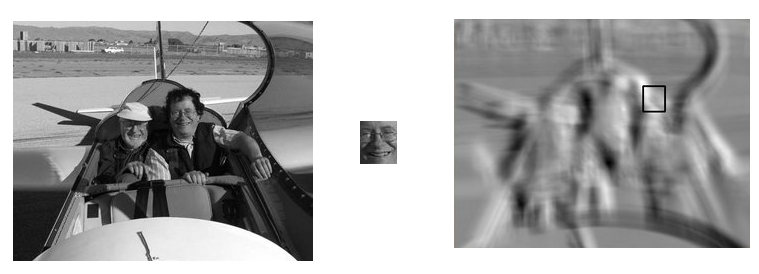
\includegraphics[width=\textwidth]{templatematching.png}
	\caption[Template Matching]{In the picture on the left, the template in the middle is to be found. Depicted on the right is the resolution matrix with potential findings indicated with the bright color and the found area of the template in the original image.~\cite{OpenCV-Documentation2018Template2018}}
	\label{templatematching}
\end{figure}

Especially in the last decade, 6D pose estimation gained popularity (\cite{Drost2010ModelRecognition}, \cite{Sundermeyer2018ImplicitImages} \cite{Hinterstoisser2013ModelScenes}). In 2018, Hodaň benchmarked 15 ODMs which share the approach of two-phased pose detection~\cite{Hodan2018BOP:Estimation}. He categorized the methods in template, point-pair-feature, local-feature and learning-based. His evaluation showed that point-pair-feature-based methods currently perform best measured against a pose-error function that deals with pose ambiguities.

To summarize, pose detection is generally split into a preparation and a detection phase. When designing a framework dealing with quickly changing ODMs, this ODM-agnostic process description should be taken into account.

\section{Service-Oriented Architectures}
SOA is a software design paradigm which gained importance towards monolithic approaches. Its main advantages over monolithic approaches are scalability, decoupling of components and simple development, testing and deployment~\cite{Richards2015MicroservicesArchitecture}. Services are concise, decoupled components capable of one specific task~\cite{Newman2015BuildingMicroservices}. The goal is to design services for maximum reusability. Together, either orchestrasted or choreographing, they form an application.

The following subsections focus on how services can be interfaced and deployed.

\subsection {Service Interfaces}
\label{serviceinterfaces}
In this section, potential client-server-based interfaces and underlying protocols shall be discussed. The evaluated interfaces are \textit{Advanced Message Queuing Protocol} (AMQP), \textit{Message Queuing Telemetry Transport} (MQTT), \textit{Representational State Transfer} (REST), \textit{Google Remote Procedure Calls} (gRPC), \textit{Graph Query Language} (GraphQL) and \textit{Open Platform Communication Unified Architecture} (OPC UA).

\subsubsection{AMQP and MQTT}
Both AMQP 0.x and MQTT are broker based protocols specialized for machine-to-machine (M2M) communication. Clients can be sensors, programmable logic controllers, etc.; the server is a broker connecting the clients. A broker is a central instance mediating between parties. Clients can subscribe to various message queues called topics. Telemetry data can then be published and read from these topics handled by the broker. The clients dynamically change between publisher and subscriber. Figure~\ref{MQTT} illustrates the MQTT architecture.~\cite{Banks2014MQTT2018}

\begin{figure}[ht]
	\centering
  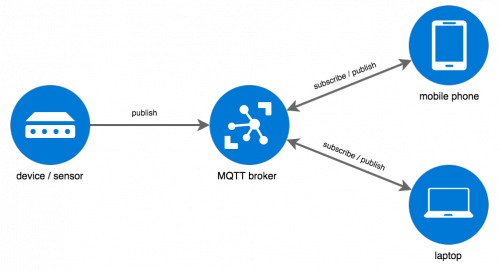
\includegraphics[width=0.9\textwidth]{MQTT.png}
	\caption[MQTT Architecture]{MQTT Architecture with the broker in the middle as a mediator between the clients~\cite{1Sheeld2018Pure-javascript-MQTT-broker.2018}.}
	\label{MQTT}
\end{figure}

A commonly used message broker is RabbitMQ which supports AMQP 0.x natively and MQTT via a plugin~\cite{RabittMQ-Documentation2018Which2018}.

AMQP needs to be distinguished between version 0.x and 1.0, as the underlying messaging paradigm has been completely revised. While for 0.x strict publishing/subscription messaging is required, version 1.0 is based on a peer-to-peer connection where a broker is not required, although possible. Due to the more sophisticated version of AMQP 1.0, fewer implementations exist.~\cite{Dizdarevic2019AIntegration}

\subsubsection{REST}
REST is an architectural paradigm describing how distributed systems can communicate with each other. It consists of five mandatory- and one optional restriction/s. If any of the five mandatory restrictions is violated, an architecture cannot be RESTful. The restrictions are client–server architecture, statelessness, cacheability, layered system, uniform interface and code on demand (optional). Roy Fielding developed REST alongside HTTP/1.1 and although it is not dependent on it, HTTP/1.1 is the primarily used protocol to implement REST. Thus, many web pages fulfill these restrictions naturally. REST messages are usually human-readable JSON files. Unlike MQTT or AMQP 0.x, REST does not rely on a broker.~\cite{Fielding2000ArchitecturalArchitectures}

\subsubsection{gRPC}
\label{sec:grpc}
For many cases in the past, it was hard for maintainers to adhere to all REST principles due to its strict nature. Moreover, REST is usually implemented with HTTP/1.1. In 2015, HTTP/2 was released to address the flaws of its predecessor~\cite{Sayfan2018REST2018}. Among those are the lack of ability of constant data streaming and latency issues.

gRPC, a remote procedure call technology introduced by Google in 2016, entirely takes advantage of HTTP/2 and thus has some advantages over REST: it allows multiplexing, binary (i.e., quick) data transfer and more. The technology behind gRPC is a remote procedure call, letting the user call remote methods as if they were local, albeit the remote method can be processed on a different hardware or system. gRPC uses protofiles to describe interface semantics. In protofiles, the user specificies service- and method names as well as message types and input/output values. Out of these protofiles, stubs can be generated which are placeholder classes for gRPC clients and servers. Unlike in most implementations of REST, gRPC does not use textual transport data like JSON but relies on Protobuf (short for protocol buffer), a binary buffer~\cite{Google-Cloud-Documentation2018Cloud2018}. For backwards compatibility towards older clients, there is a gateway available which provides transcoding from HTTP/JSON to gRPC. See figure~\ref{ESP} for the concept behind it~\cite{gRPC-Gateway-Documentation2017Grpc-gateway.2018}.

\begin{figure}[ht]
	\centering
  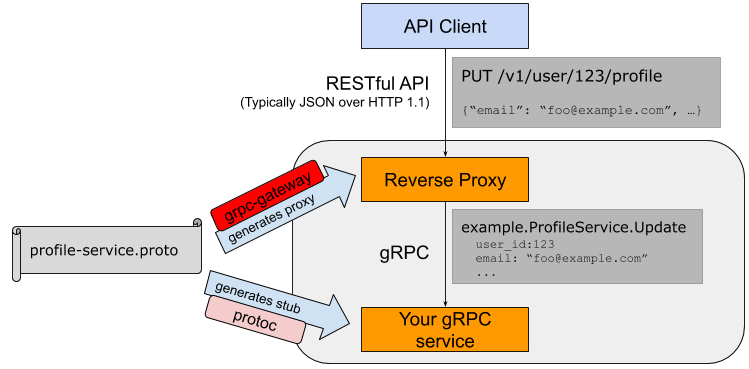
\includegraphics[width=\textwidth]{img/grpc_gateway.png}
	\caption[gRPC gateway concept]{gRPC gateway concept~\cite{gRPC-Gateway-Documentation2017Grpc-gateway.2018}. Based on a protofile, it generates a reverse proxy which handles RESTful API client requests and maps them to gRPC methods.}
	\label{ESP}
\end{figure}

The gateway is a plugin of protoc (short for protocol compiler) as part of gRPC's ecosystem. Based on a given proto file, the gRPC-gateway generates a reverse proxy offering a RESTful interface which internally maps REST/HTTP1.1 to gRPC calls. The mapping between gRPC and HTTP is described here with an example protofile directly quoted from Google's API documentation~\cite{Google-API-Documentation2019Http.proto.2019}:\\

\begin{lstlisting}[language=protobuf3,style=protobuf]
     service Messaging {
       rpc GetMessage(GetMessageRequest) returns (Message) {
         option (google.api.http) = {
             get: "/v1/{name=messages/*}"
         };
       }
     }
     message GetMessageRequest {
       string name = 1; // Mapped to URL path.
     }
     message Message {
       string text = 1; // The resource content.
     }
\end{lstlisting}

The option in the protofile enables HTTP REST to gRPC mapping:

    \begin{tabular}{c|c}
        \textbf{HTTP} & \textbf{gRPC} \\ \hline
        GET /v1/messages/123456 & GetMessage(name: "messages/123456")
    \end{tabular}

\subsubsection{GraphQL}
GraphQL is a data query and manipulation language. It was developed by Facebook and is open-source since 2015. Compared to REST, it has a more flexible and efficient approach. The increase in efficiency over REST is based on faster mobile data access, and more flexibility for the application programming interface (API) to let clients access precisely the data they need, i.e., the server modifies the data with respect to the clients' needs instead of providing one rigid resource. REST allows the user to pass a single set of arguments - the query parameters and URL segments. In GraphQL, every field and nested object can get its own set of arguments. It also lets the user pass arguments in scalar fields allowing for data transformations. An example query directly quoted from GraphQ's documentation is depicted here~\cite{GraphQL-Documentation2018Basics2018}:

\begin{lstlisting}
 {
  human(id: "1000") {
    name
    height(unit: FOOT)
  }
}
\end{lstlisting}

The corresponding response from the server is:

\begin{minipage}{\linewidth}
\begin{lstlisting}
 {
  "data": {
    "human": {
      "name": "Luke Skywalker",
      "height": 5.6430448
    }
  }
}
\end{lstlisting}
\end{minipage}

\subsubsection{OPC UA}
OPC UA is a \textit{machine-to-machine} (M2M) protocol specialized in vendor independent communication between heterogeneous machines. Until 2018, there were two means of data exchange available for OPC UA: binary data over transmission control protocol (TCP) or extended markup language (XML) data over \textit{Simple Object Access Protocol} (SOAP). Due to the higher performance, the former is primarily used nowadays.~\cite{Schleipen2016OPCVariability} 

In 2018, the OPC Foundation introduced part 14 of the OPC UA specification stack, OPC UA Publish/Subscribe~\cite{OPC-Foundation2018OPC1.04}. It is used to communicate messages between different system components without these components having to know each other’s identity. Now it is possible to use more protocols for data exchange: AMQP, MQTT, OPC UA user datagram protocol (UDP) and OPC UA Ethernet. OPC UA UDP can perform multicasts, i.e., one entity can send data to a group with the same effort as sending to a single entity. Multicasts are more performant than brokers, although do not enable time decoupling of services~\cite{Eckhardt2018AnCases}. OPC UA Ethernet is a simple Ethernet based protocol not relying on IP or UDP~\cite{OPC-Foundation2018OPC1.04}. As for the payload of the protocols, JSON or UADP are allowed. UADP is specialized for cyclic communication between, e.g., PLCs. The payload is included directly in the transport protocol.

Eckhardt et. al. performed an evaluation based on expert estimates in 2018 on how the different combinations of data exchange in OPC UA suit for the specific needs at the field, control, human-machine-interface (HMI) and enterprise level~\cite{Eckhardt2018AnCases}. See figure~\ref{fig:opc_ua_dataexchange} for an overview for the evaluated combinations.

\begin{figure}[ht]
    \centering
    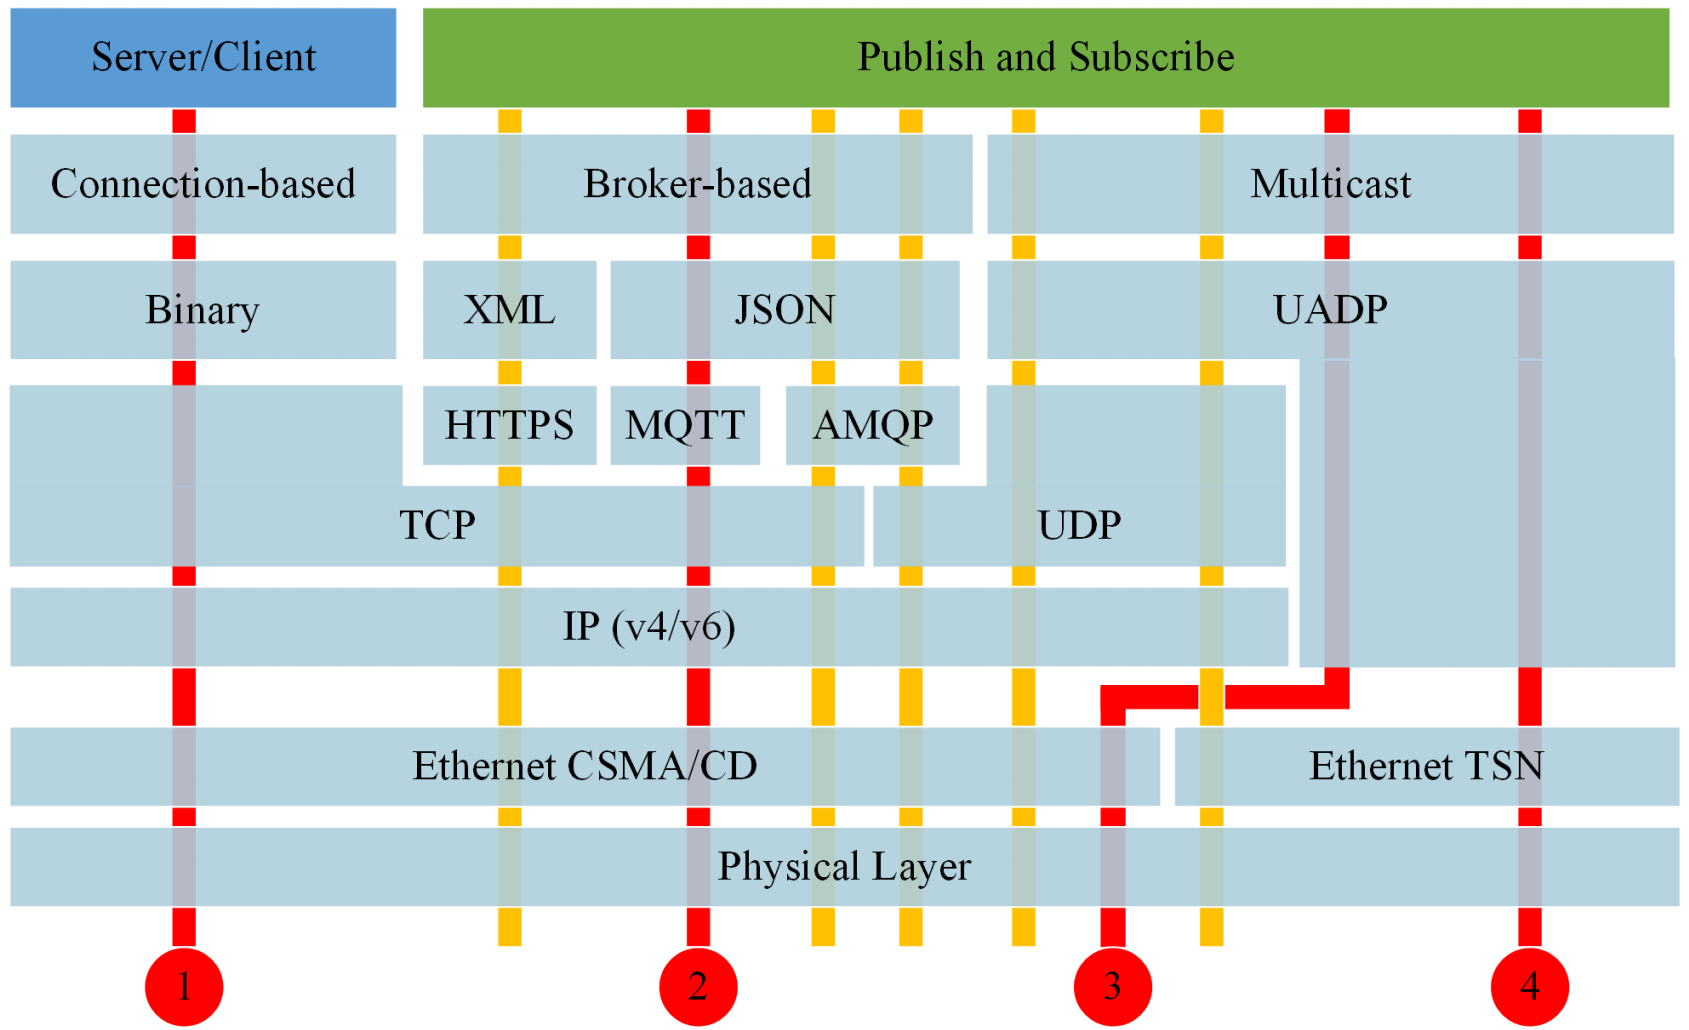
\includegraphics[width=\textwidth]{img/OPC_UA_Data_Exchange.png}
    \caption[OPC UA Data Exchange Variants]{OPC UA data exchange variants. The red and yellow vertical lines are possible variants, the red lines are evaluated in detail in~\cite{Eckhardt2018AnCases}.}
    \label{fig:opc_ua_dataexchange}
\end{figure}

The experts estimated that all combinations are suitable for HMI and enterprise level, but only combinations 3 and 4 are suited for control and field level. Combination 4 uses OPC Ethernet TSN which is OPC UA's approach of eliminating the need for fieldbus protocols~\cite{Wilmes2019ZauberwortKonvergenz}. TSN resides on OSI reference model layer 2 as a set of standards\footnote{mainly IEEE 802.1Q~\cite{2018IEEENetworks}. See~\cite{Bruckner2019AnSystems} for a full list and detailed description.} to boost ethernet networks with low latency and high availability. So-called \textbf{convergent} networks can be implemented with TSN, meaning different components (sensors, PLCs, etc.) can each arrange data streams - from synchronous low-latency to event-based. Streams can be extended or altered at any time. The main components of TSN are time synchronization enabling real-time functionalities, and scheduling and traffic shaping enabling coexistence for multiple streaming classes. \\
In practice, there are some network adapters and switches available which implement a subset of the TSN standards. The open-source automation development lab which is also responsible for the open-source project open62541\footnote{An implementation of OPC UA under the Mozilla public license 2.0 as opposed to the dual license model (i.e., proprietary for members, general public license 2.0 for non-members) of the OPC Foundation~\cite{Emde2019DieLizenzen}.} currently evaluates performance and prices of the released hardware~\cite{Emde2019DieLizenzen}. While a user currently has to accept a price increase of 1000-2000\,\% as opposed to conventional hardware, the tests confirm TSN to be as performant as established fieldbus systems~\cite{Emde2019DieLizenzen}.

There was also an attempt to create an OPC UA to REST adapter by Ronnhölm in 2018~\cite{Ronnholm2018IntegrationThesis}. Although OPC UA allows HTTP on the application layer, there is an incentive: OPC UA is not RESTful. RESTful HTTP is centered around resources that can be identified by a URL and a message. Any body of data may therefore be manipulated independently of any intermediary application logic. This is not the case with HTTP in OPC UA. Ronnhölm claims (\cite{Ronnholm2018IntegrationThesis},~page 26): \say{To enable exchange with OPC UA servers without the use of an OPC UA stack, a holistic translation must translate both structural and foundational aspects of OPC UA. This means that translation must bypass OPC UA transport protocols, secure channel management, serialization and OPC UA services - all in a way that avoids semantic dependencies and preserves translation transparency.} He concludes that a subset of OPC UA services can be transformed to REST when combined with standard create-request-update-delete methods.

\subsection {Deployment Options}
\label{deploymentoptions}
In the last decades, most software applications had a monolithic character which did not focus much on scalability and agile development. With the progress in digitalization, applications had to become more flexible and faster. To address the challenge of deploying applications highly automated, container architectures came about. Unlike virtual machines which need an operating system, runtime and system variables to operate well, Docker and other virtualization technologies are sandbox systems which can imply all the mentioned features and furthermore can run on almost any operating system. In the following, two possible virtualization technologies are briefly introduced, namely Heroku and Docker. They are motivated by pointing out how they are superior to virtual machines in the context of microservices.~\cite{Wurbs2017Docker2018.}

Docker is an open-source standard for operating-system-level virtualization. If Docker is installed on an operating system, it is possible to run several applications on the machine simultaneously, with low start and stop times and little overhead. These applications can rely on different platforms, dependencies, runtimes, etc. The technology behind it is a daemon which shares low-level components with the host operating system. A hypervisor is not necessary (see figure~\ref{container} for an illustration). 

\begin{figure}[ht]
	\centering
  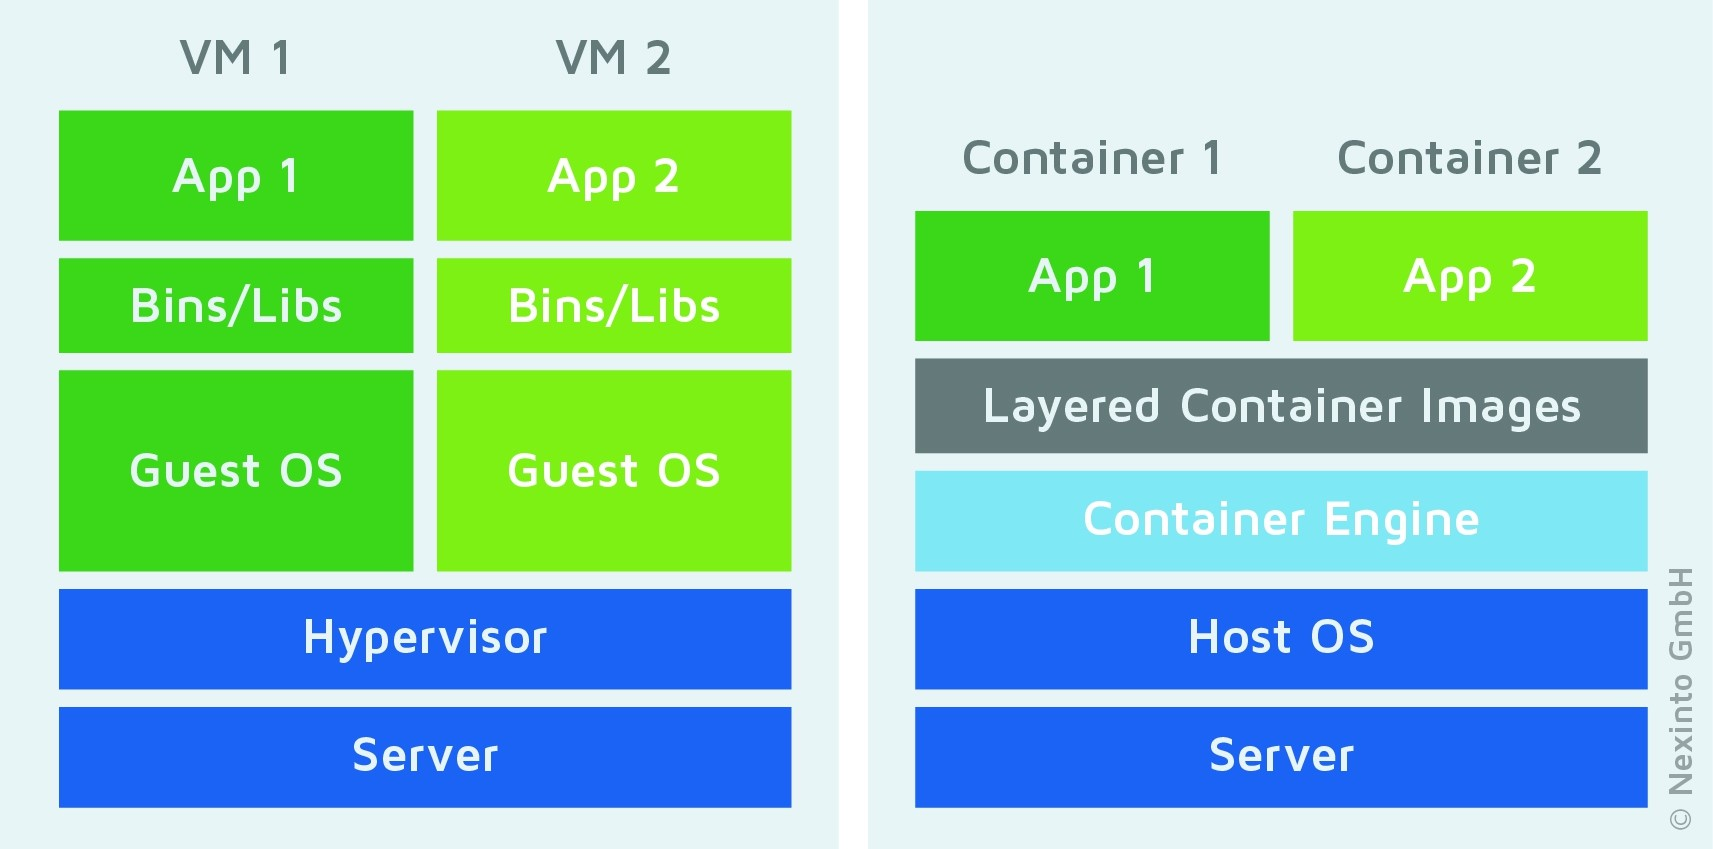
\includegraphics[width=0.7\textwidth]{containervsvm.jpg}
	\caption[Docker vs Virtual Machine Architecture]{Virtual machine architecture on the left versus container architecture on the right. Docker does not rely on a hypervisor.~\cite{Wurbs2017Docker2018.}}
	\label{container}
\end{figure}

To virtualize applications, Docker uses containers which are built up on Docker images. Images are read-only templates that are built from a set of instructions written in a dockerfile. They offer one great advantage - a layered file system. This enables the user to easily add or update applications very quickly. Images can be shared in a public/private registry called Docker Hub. \\
Last but not least, development and operations of applications can be harmonized through a combination of Docker and a continuous integration and continuous delivery platform. 

Heroku is a platform as a service provider whose underlying technology shares some core concepts with Docker. E.g., BuildPacks are a set of scripts which are used to set up the final state of an image. The pendant on the Docker side is called dockerfile (see Thurig's blog~\cite{Thurig2014Docker2018} for a full description of the similarities and table~\ref{dockerandheroku} for a list of pendants). However, there are also differences between the two alternatives. The main one is the dependency on the Heroku platform on the Heroku side, whereby on the Docker side one is completely flexible in choosing any environment from Raspberry Pi to cloud platform providers like Amazon Web Services. The latter also means a surplus of workload on infrastructure on the Docker side. Also, one is less flexible on the prices. Heroku has a staged price model ranging from 0 to 500\,\$ per month and dyno. Docker is again more flexible in letting one just paying for the hosting and storaging and leaving the additional features provided by Heroku aside.~\cite{Chris2017Why2018} 


\begin{table}
\begin{center}
      \caption[Similar core concepts of Docker and Heroku]{Similar core concepts of Docker and Heroku. \cite{Thurig2014Docker2018}}
  \begin{tabular}{ l | l }
    Docker & Heroku  \\ \hline
Dockerfile &	BuildPack \\ 
Image	& Slug\\ 
Container&	Dyno\\ 
Index	&Add-Ons\\ 
CLI	&CLI
  \end{tabular}
  \label{dockerandheroku}
\end{center}
\end{table}

\section{Object Detection Service Interface Semantic}
If two humans want to communicate with one another, they need matching channels and need to speak the same language. A channel is a mean of transport for information, e.g., sign language, smoke signs and mobile phones. If one entity tries to call someone via phone if the other does not have a phone or the caller enters the wrong number and the other has its cellphone turned off, they cannot communicate. In case they both have a phone, the called entity answers and both speak a common language (e.g., English), the exchange of information can be achieved. Communication within technical systems faces the same challenges. As for the right channel, models like the open systems interconnection (OSI) basic reference model for information technology standardized by the international organization for standardization (ISO) layer the transfer of information. It ranges from the physical layer consisting of peaks in currents and voltages up until the application layer which includes direct user interaction, resource availability and so forth~\cite{InternationalOrganizationForStandardization1996ISO/IECEd.}. This model and the protocols adhering to it ensure that information is delivered safely between communicating entities. However, this model does not imply the semantics of the payload or the language, as stated in the analogy above. 

This section introduces two possible ways of how an ODS service interface semantic can be designed. One resides in the IT and cloud domain whereas the other rather resides in the OT domain.

\subsection{Google Cloud Vision API}
Google Cloud Vision (GCV) API offers a publicly available REST and gRPC interface~\cite{Google-Cloud-Documentation2019Google2019-04-26}. OD operations can be executed on the cloud. The upside of this approach is excessive computing power and an attractive pay-per-use price model. The downside is the limitation of the configurability of Google's ODs and the lacking transparency of where and how the data is stored and evaluated. An example gRPC call for annotating images with labels of objects is depicted here:

\begin{lstlisting}[language=protobuf3,style=protobuf]
    rpc AsyncBatchAnnotateFiles(AsyncBatchAnnotateFilesRequest) returns (Operation)
\end{lstlisting}


\subsection{OPC UA Vision}
A currently proposed semantic standard for OD processes is \textbf{OPC UA Vision}. It includes a finite state machine abstracting an industrial system from its diverse conditions and transitions. Moreover, it offers an information model covering the administration of recipes, configurations and results. With the help of the state machine, it is defined which information of the information model is retrievable. The content of the three administration objects remains proprietary with the advantage of covering a broad range of OD scenarios.

\subsubsection{State Machine}
According to the specification, powering up and shutting down a vision system are mandatory processes and thus should be handled in a standardized manner. Also, the handling of errors should be the same for all vision systems. The design of the core operation state, however, shall remain with the manufacturer. Automatic mode as a sub-state of operational mode is one proposed way of designing it. The state machine for a typical vision system in automatic mode is depicted in figure~\ref{fig:OPCStateMachineAutomatic}. An example of this operation would be a PLC guiding an inspection system for position determination. When powered on, the system enters the preoperational state through loading a configuration marked as active. From there, an operation mode is either automatically chosen by the system or manually triggered. An operation mode is any sub-state machine of the operational state. The automatic mode is chosen and enters the initial state. Then a recipe can be prepared, describing properties, procedures and parameters for a machine vision job. The recipe may include information for a single and/or continuous execution. A single execution would be e.g. determining the pose of an object; a continuous execution could be monitoring and surveillance systems which constantly process and acquire data. When the system is done with an execution or execution step, e.g., taking a picture from one of four angles, it sends results asynchronously to the client. If the system is shut down, it should be put into halt mode first where a safe power-off is assured. From all states, it is possible to enter the error state. Errors are handled aligning with their severity and sometimes need acknowledgment or confirmation by a human before the system can be reset to preoperational state.

\begin{figure}[ht]
    \centering
    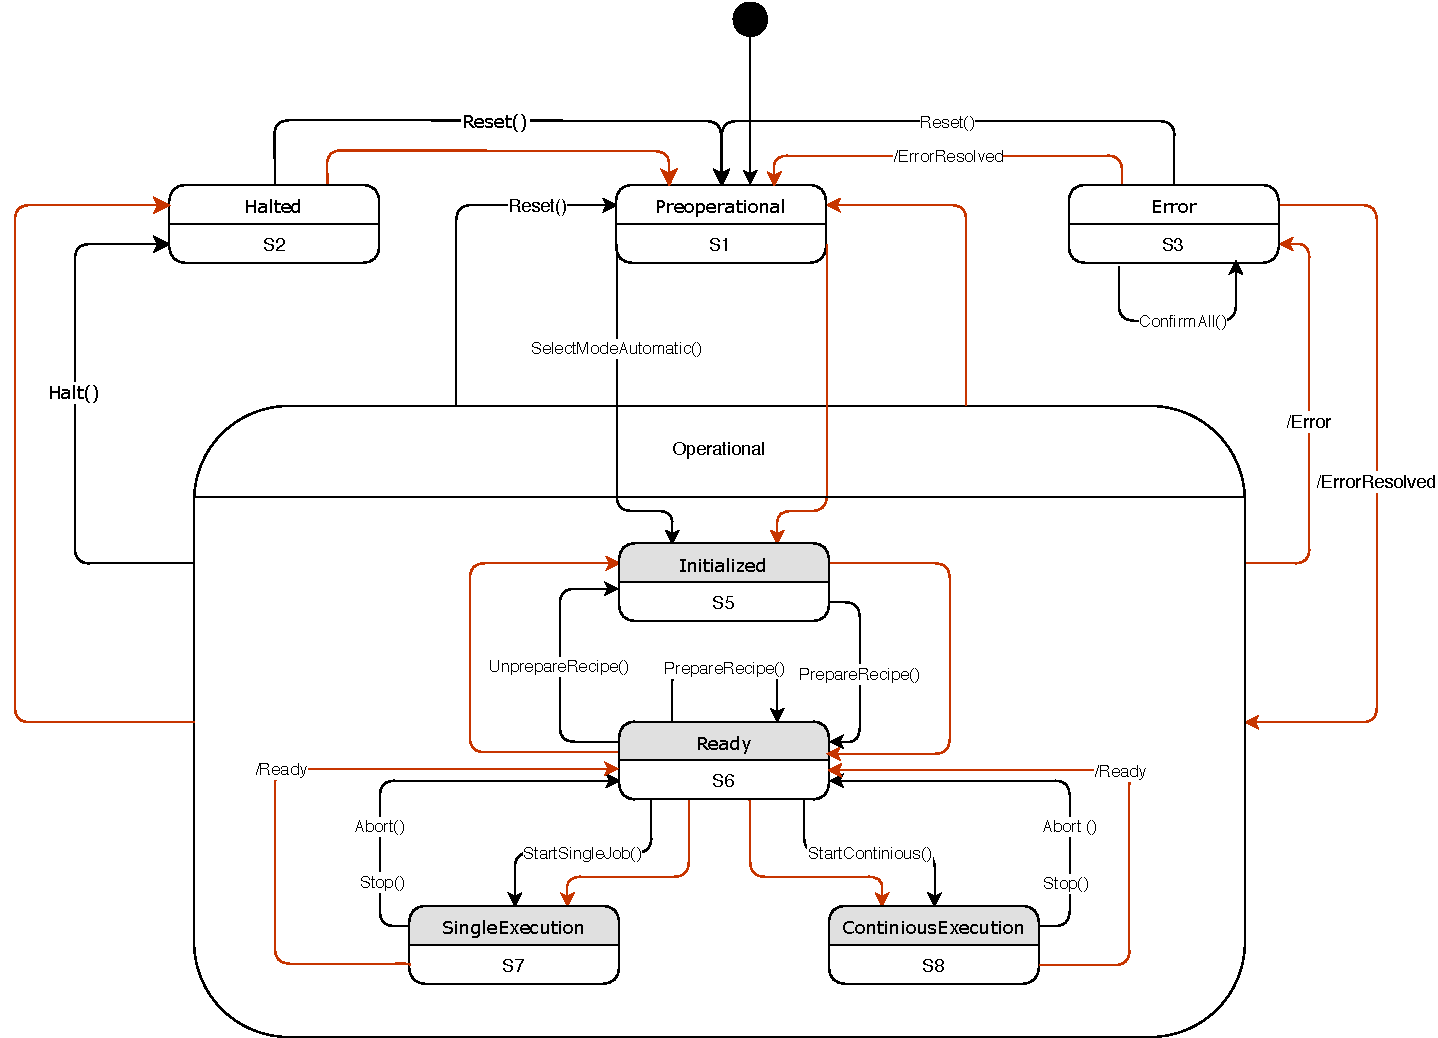
\includegraphics[width=\textwidth]{img/OPCUAVisionVisionAutomaticModeStateMachineStates.pdf}
    \caption[OPC UA Vision state machine in automatic operation mode]{OPC UA Vision state machine in automatic operation mode. Red Lines indicate automatic transitions induced by the vision system with optional effects prefixed with a slash. Black lines indicate method induced transitions with the method name as the trigger. The black circle is the entry point of the state machine. All of the states can have optional sub-state machines. States marked in grey are substates.~\cite{VDMA2018OPC40100-1:2018-11}}
    \label{fig:OPCStateMachineAutomatic}
\end{figure}

\subsection{Information Model}
The information model formally describes all datasets, types, methods, address- and namespaces. See figure~\ref{fig:OPCInfoModelOverview} for an overview and figure~\ref{fig:OPCInfoModelNotation} for an explanation of the notation. Configuration, recipes and result are the three types that have to be dealt with when using OPC UA Vision.

\say{Even identical vision systems may vary in some details. In order to produce the same results the vision systems have to be adjusted individually e.g., calibrated. Within this document, the set of all parameters that are needed to get the system working is called a configuration. Configurations can be used to align different vision systems that have the same capabilities, so that these systems produce the same results for the same recipes. The ConfigurationManagement handles all configurations that are exposed by the system. Only one configuration can be active at a time. This active configuration affects all recipes used in the machine vision system.}~(\cite{OPC-Foundation2018OPC1.04}, chapter~7.2)

\say{Properties, procedures and parameters that describe a machine vision task for the vision system are stored in a recipe. Usually there are multiple usable recipes on a vision system. This specification provides methods for activating, loading, and saving recipes. Recipes are handled as binary objects. The interpretation of a recipe is not part of this specification. Recipes are potentially complex entities. A recipe may contain (possibly nested) references to sub-recipes and it may be used for several products. The internal composition of recipes – including the referencing of sub-recipes – is outside the scope of this specification.}~(\cite{OPC-Foundation2018OPC1.04}, appendix~1.2.1 and~1.2.2) For an example recipe life cycle, see appendix~\ref{chap:recipelifecycle}.

\say{ResultManagementType provides methods to query the results generated by the underlying vision system. Results can be stored in a local result store.}~(\cite{OPC-Foundation2018OPC1.04}, chapter~7.8)

XML nodesets can be used to import information models to an OPC UA server. A screenshot of an example information model uploaded to an OPC UA demo server and viewed by UAExpert is depicted in~\ref{fig:uaexpert}. It also shows how methods are called, in this example a simple product of two numbers. An important, more sophisticated method of the OPC UA Vision specification is StartSingleJob (subpart of StateMachineType, not depicted in the information model overview in~\ref{fig:OPCInfoModelOverview}). Usually it is called by a PLC to trigger a machine vision task. Its signature consists of following parameters:

\begin{minipage}{\linewidth}
\begin{tabbing}
    space \= space \= spacespacespace \= spacespacespacespace \= spacespacespace \kill
    \>  StartSingleJob(\\
    \>  \>  (in)	 \> 	String          \> MeasId\\
    \>  \>  (in)	 \> 	String          \> PartId\\
    \>  \>  (in)	 \> 	RecipeIdType    \> RecipeId\\
    \>  \>  (in)	 \> 	ProductIdType   \> ProductId\\
    \>  \>  (out)	 \> 	String          \> JobId\\
    \>  \>  (out)	 \> 	Int32           \> Error); 
\end{tabbing}
\end{minipage}

In another section of the specification, the data types are defined, e.g. RecipeIdType, which is a structure including an Id, a version and a hash.

When the method is called, it triggers transition from state Ready to SingleExecution in the state machine as depicted in~\ref{fig:OPCStateMachineAutomatic}.

\begin{figure}[ht]
    \centering
    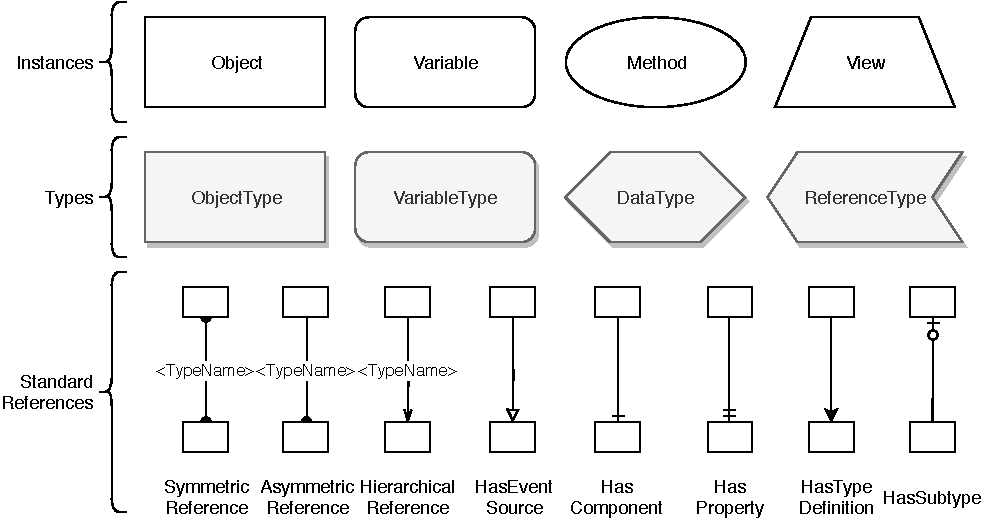
\includegraphics[width=0.8\textwidth]{img/OPCUAVisionInformationModelNotation.pdf}
    \caption[OPC UA Vision Information Model Notation]{OPC UA Vision Information Model Notation.\cite{VDMA2018OPC40100-1:2018-11}}
    \label{fig:OPCInfoModelNotation}
\end{figure}

\begin{figure}
    \centering
    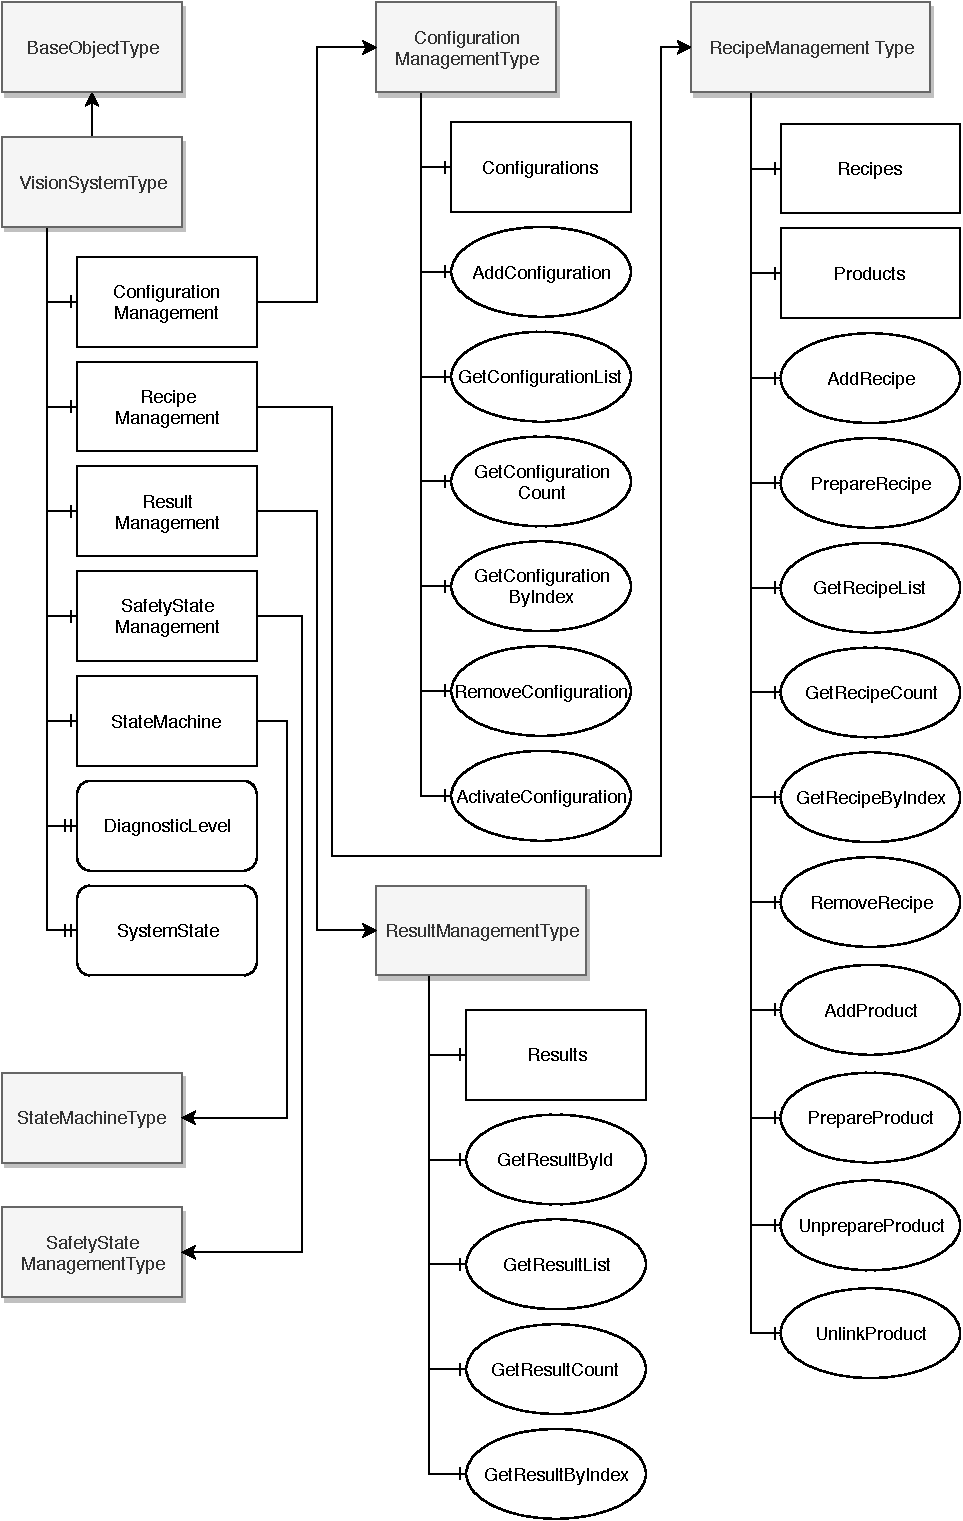
\includegraphics[height=0.9\textheight]{img/OPCUAVisionInformationModelOverview.pdf}
    \caption[OPC UA Vision Information Model Overview]{OPC UA Vision Information Model Overview. See fig. \ref{fig:OPCInfoModelNotation} for a description of the notation.~\cite{VDMA2018OPC40100-1:2018-11}}
    \label{fig:OPCInfoModelOverview}
\end{figure}

\begin{landscape}
\begin{figure}[ht]
    \centering
    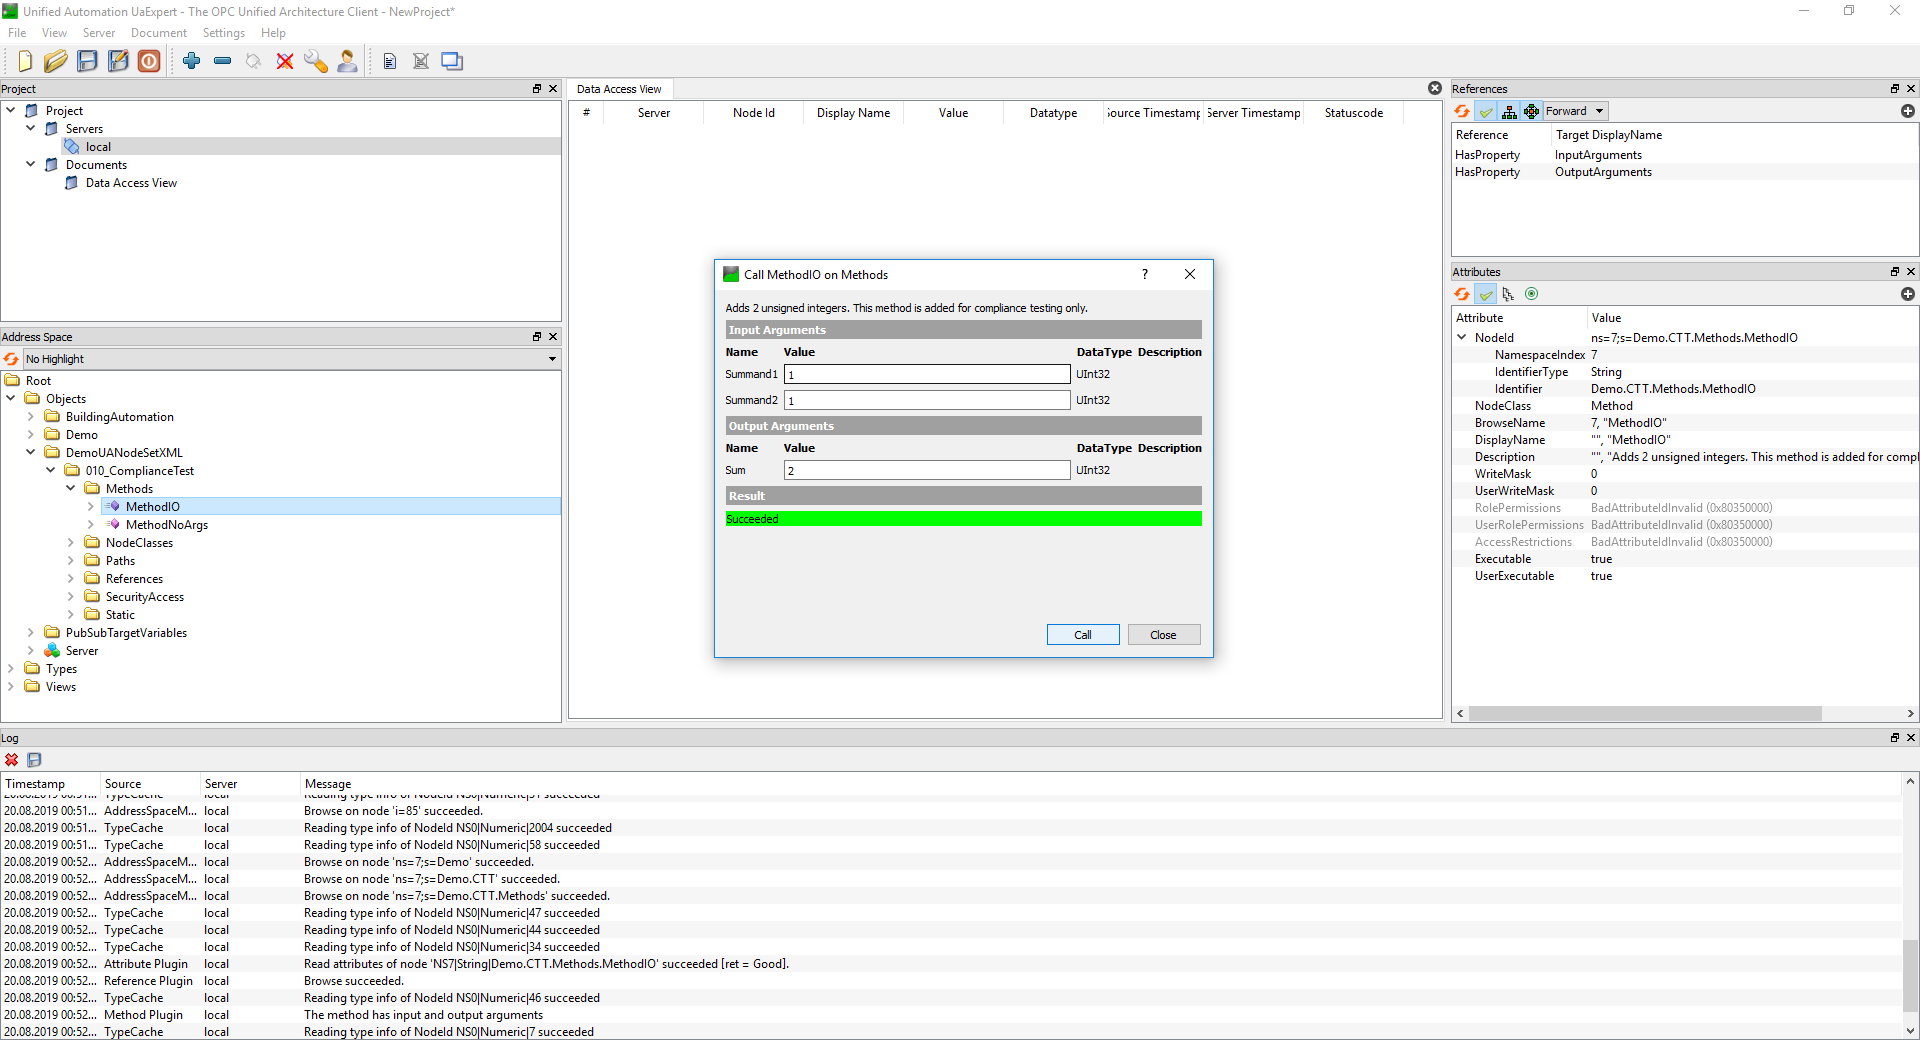
\includegraphics[width=1.5\textwidth]{img/UAExpertScreenshot.png}
    \caption[Example Information Model in UAExpert]{Screenshot of UAExpert showing an example information model in the folder hierarchy on the left. The data access view in the middle is a list of nodes and their corresponding current values. Also, a simple method call multiplying two values is depicted on the bottom right corner. The multiply method implies references and attribute which are pointed out on the right.}
    \label{fig:uaexpert}
\end{figure}
\end{landscape}

\section{Summary}
The most important aspects of the state of the art sections are:
\begin{itemize}
    \item Contemporary ODM use 3D and RGB-D images for pose determination in \textbf{two phases}.
    \item Service interface protocols have to be chosen appropriately for every application.
    \item Containerization is a convenient way of deploying services.
    \item OPC UA Vision is based on an information model and a state machine based on which is decided which information is retrievable.
    \item Recipes are vendor-specific.
\end{itemize}

    \chapter{Industrial ODS Concept\label{cha:chapter3}}

In this concept the ODS is a recipe for an OPC Vision server. See fig. \ref{fig:concept} for an overview. 
\begin{figure}
    \centering
    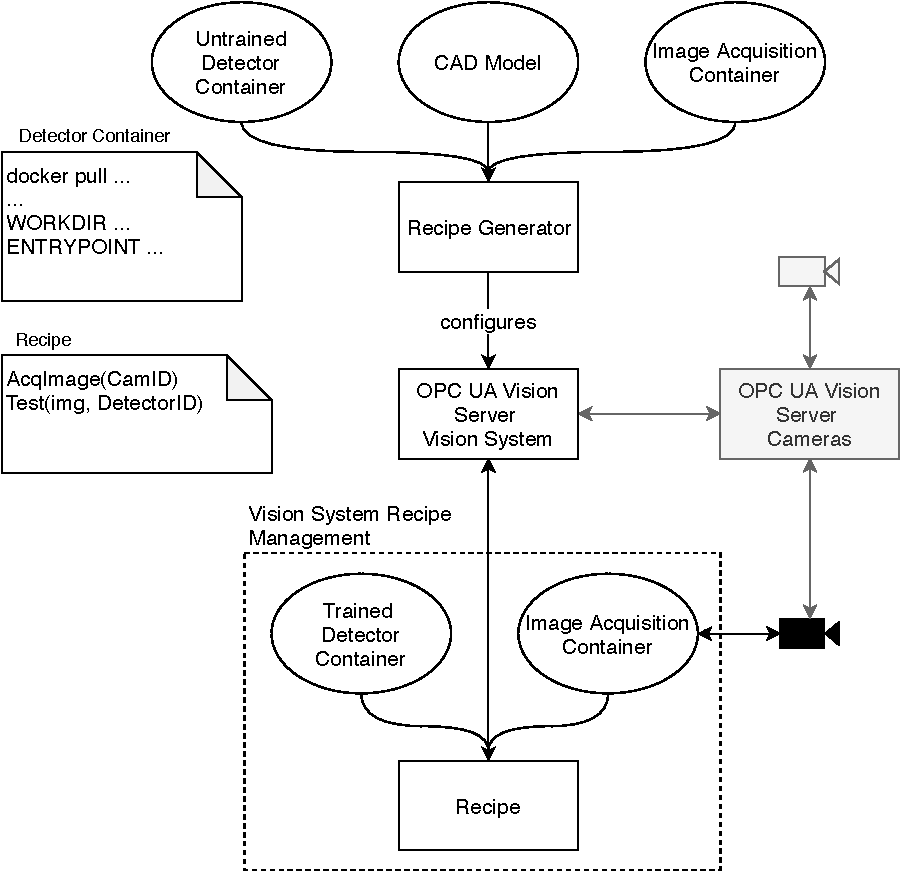
\includegraphics[width=\textwidth]{img/Concept.pdf}
    \caption[Concept]{Illustration of the industrial ODS concept. Ellipses denote inputs, solid rectangles systems, dotted rectangles scopes of systems and notes the content of a file. The OPC UA Vision server for cameras is not yet released by the OPC foundation, hence marked grey.}
    \label{fig:concept}
\end{figure}

The ODS is a trained detector container which is generated with a CAD model and an untrained detector as input. The detector must provide two methods:
\begin{tabbing}
\label{detectormethods}
    space \= space \= spacespacespace \= spacespacespacespace \= spacespacespace \kill
    \>  Train(\\
    \>  \>  (in)	 \> 	CADType          \> CADModel); \\
    \>  Test(\\
    \>  \>  (in)	 \> 	ImageType     \> Image\\
    \>  \>  (out)	 \> 	PoseType           \> Pose); 
\end{tabbing}

Train is a training routine which generates several views or templates from a CAD model. It must be preconfigured by the detector provider e.g. learning rates of neural networks have to be preset. After training the detector container includes generated templates or views and is callable with the Test method.  Test requires an image for processing the pose of an object aided by the generated templates.  Input and output types are not specified in this thesis. The container is illustrated as a Docker image, this is not mandatory however.

The detector container is added to recipe management of the VS via OPC UA Vision server. Recipes are scripts which handle image acquisition- and detection container calling and OPC UA Vision server interaction. Scripts can be added by the recipe generator or another entity. Image acquisition is currently set to be handled between image acquisition containers and cameras directly. This might change in the near future. During a phone interview conducted on 30th of April 2019, VDMA member Dr. Reinhard Heister stated that part 2 of the OPC Vision specification will direct the component layer. A component can be a camera that offers an OPC Vision server itself. For this task, OPC foundation and EMVA, supervisor of the GenICam interface \cite{LastvisitedMay4th20192019GenICamStandard} for cameras, will join forces. Hence in a few years time it will be possible to have the VS to be interoperable with any camera supporting OPC Vision and the images can be acquired via the OPC servers.


\section{Sequence Diagram}
Figs. \ref{fig:runtimeviewgen} and \ref{fig:runtimeviewexec} show an example sequence diagram of the service generation, transfer and execution. The approach is as follows:
\begin{figure}
    \centering
    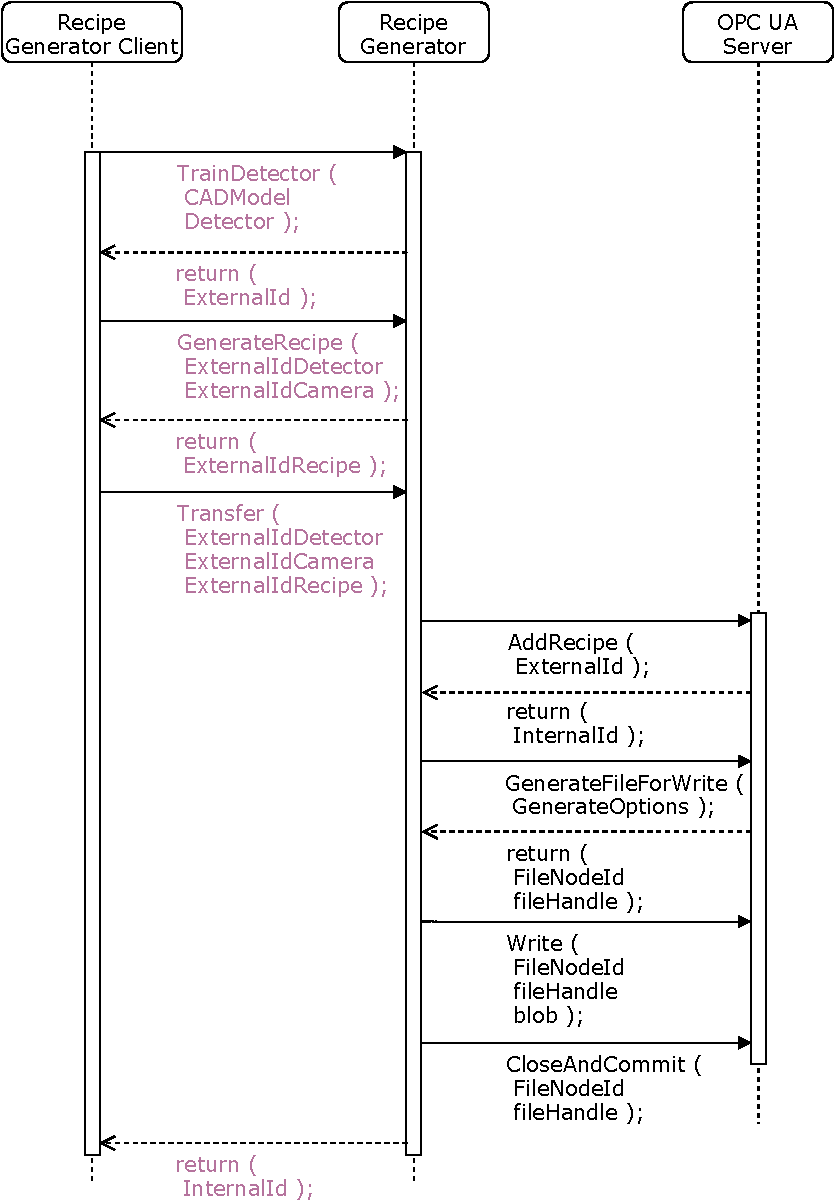
\includegraphics[height=0.9\textheight]{img/ConceptRuntimeView-RecipeGenerationAndTransfer.pdf}
    \caption[Sequence diagram recipe generation and method based transfer]{Sequence diagram of recipe generation and method based transfer to OPC UA Vision server. Pink arrows denote methods which are not covered by OPC Vision specification. Not all parameters of method signatures are shown.}
    \label{fig:runtimeviewgen}
\end{figure}

\begin{figure}
    \centering
    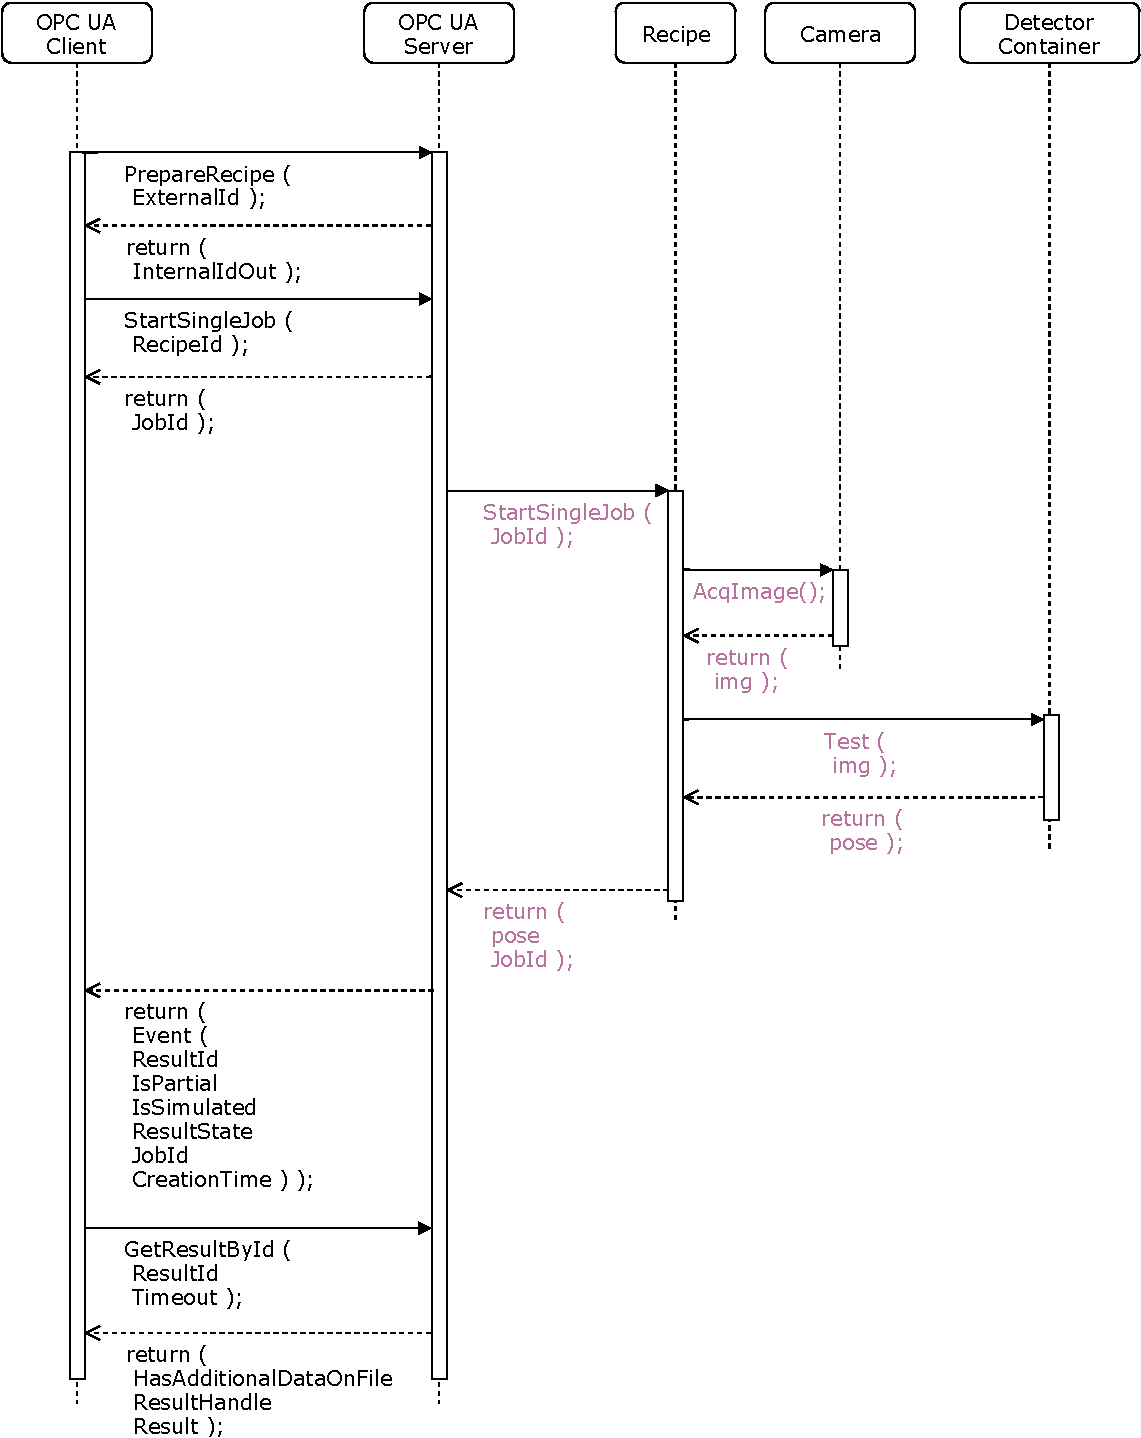
\includegraphics[height=0.9\textheight]{img/ConceptRuntimeView-RecipeExecution.pdf}
    \caption[Sequence diagram of recipe execution]{Sequence diagram of recipe execution of method based OPC UA Vision server. Pink arrows denote the recipe which is not covered by OPC Vision specification. Not all parameters of method signatures are shown.}
    \label{fig:runtimeviewexec}
\end{figure}

\begin{itemize}
    \item Generation and Transfer
    \begin{itemize}
        \item TrainDetector trains the detector with the Train method using a CAD model as input. The detector service changes state from untrained to trained and can be called via Test method.
        \item GenerateRecipe puts image acquisition and detector into sequence. Hence, when triggered an image is grabbed, passed to the Test method of the detector, which output the pose of the object in the image.
        \item Transfer initiates detector, image acquisition or recipe transfer. The object to be transferred is identified with the ExternalId.
        \item AddRecipe creates a new recipe opject and maps an InternalId to the ExternalId. ExternalId is an OPC UA datatype identifying a recipe in the view of the environment, InternalId is an OPC UA data type identifying an instance of the recipe on the VS.  InternalId is necessary because recipes can not only be handled via the server but also locally on the VS. For the OPC UA client, only the ExternalId should be callable and internal ambiguities must be handled by the VS. The created recipe object can contain meta data of the recipe and a reference to the recipe itself. As of now, it contains no data.
    	\item GenerateFileForWrite creates a new temporary file object. The GenerateOptions parameter contains the ExternalId of the process. The method returns a FileNodeId and a FileHandle. The temporary file object offers Write and CloseAndCommit methods to transfer binary recipe data. The recipe itself is treated as a file and is referenced in the recipe object.
    \end{itemize}
    \item Execution
    \begin{itemize}
    	\item PrepareRecipe is used to prepare a recipe so that it can be used for starting a job on the vision system. There are several ways the vision system can cope with recipes and their preparation. For example, the vision system can have several recipes prepared for immediate execution or just a single one. PrepareRecipe triggers transition from state Initialized to state Ready of the VS state machine. If the client tries to prepare a detector oder image acquisition container it should return an error.
    	\item StartSingleJob method triggers transition from state Ready to state SingleExecution. Parameter RecipeId is the ExternalId of the recipe script. The method returns a JobId which has to be used to query any information about the Job later.
    	\item AcqImage triggers a camera to acquire an image. In case several cameras are addressable, the method can be overloaded with a CameraId.
    	\item Test calls the detection routine of the detector service and returns the pose an object.
    	\item Once the Train method is complete the OPC server triggers an event to the OPC client containing the JobId and ResultId. It also provides information on whether the result is partial, the job is done and when the result was created.
    	\item GetResultById is used by the client to query the template matching result via RecipeId and a timeout which aborts the transfer after a given time. It returns meta data about the result and the possible reference to result data containing e.g. the base image. In this case, the detected point can be stored in the result object itself.
    \end{itemize}
\end{itemize}

\section{Deployment}
\subsection{Vision System}
In a typical industrial environment, the VS is a production line or a single machine. According to the OPC Vision specification the application can range from simple light barriers to complex pose detection. The recipes presented here are rather designed for the latter purpose, however can be used for the former, too. On the software side, the VS has to cover recipe, configuration and result management. Depending on the size of the system (number of cameras, data storage, CPU cores...) it can be deployed on a single industrial PC or in a larger factory cloud. The detection and image acquisition services in this work are containerized microservices, so the underlying hardware must support the containerization engine. According to an interview with VDMA experts \cite{Lastvisited26-04-20192015OPCVision} more and more machine vision functionalities shall be transferred to PLCs. This might call for a different approach of deployment for the recipes in a later stage. The OPC client triggering the job / recipe execution is usually a PLC.\\

\subsection{Recipe Generator}
As for the recipe generator, there are more possibilities. Since detectors could be added by several vendors in a hub, it would make sense to make this available in a (virtual private) cloud. The recipe generation might also require excessive computing power, which can be provided by cloud platforms. Furthermore, mobile networks such as the 5G technology offer a bandwidth up to 10.000\,MBit/s and a latency under 1\,ms, so costs on the infrastructure side can be minimized. Possible drawback is the increased security need of data storage and transmission.

The generator might also be deployed as part of the vision system. The advantages of this concept are better data protection possibilities and lower latency. The drawback in this case is the lower computing power and tougher access for ODS vendors.

\section{Interfaces}
\subsection{Detector Containers}
The detector containers are called during the execution of a recipe. The services might also be called in sequence. For this communication a standardized interface is of great help. As for the semantic, the two methods Train and Test are defined. For data transport RPC is a good choice due to its high performing request calls. With the Train and Test methods defined, most of the application logic can reside inside the server (detector container), hence changes of ODM do not cause changes for the client (recipe). The connection between recipe, OPC UA Vision server and cameras is implementation specific.\\

\subsection{Recipe Generator}
The recipe generator needs an interface for the OPC UA Vision server on the one hand and on the other hand for the recipe generator client. In case the generator is deployed in an industrial environment it would be reasonable to configure not only the recipe transfer but also the recipe generation via OPC UA to maintain a great interoperability within the shopfloor. For instance, CAD models can be created by cameras and automatically sent to the recipe generator. In case it is deployed in a web environment, an interface rather developed for web technologies is advantageous. For instance RPC with a RESTful adapter could be used for that purpose.

\subsection{Image Acquisition}
As of now, the image acquisition containers do not have a standardized interface. This is due to the plans of the OPC foundation of fulfilling this task in the near future.

\section{Orchestration of Recipe Management}
The recipe, image acquisition- and  detector containers combine to recipe management of the OPC UA Vision server. As recipes handle image acquisition and detector container calling, one could say it serves as an orchestrator and is a single point of failure. A possible hazard would be applying too much application logic to the recipe, thus it should stay simple and only run necessary OD steps by calling the containers in sequence with a standardized interface. This maximizes cohesion of the components. In case putting several trained detector containers in sequence, the output of the Test method would have to be abstracted since the second and following containers would receive a pose of an object as input which is unlikely useful. Abstracting output types would again shift application logic to the recipe which should be minimized. Hence, sequencing OD containers should be scoped in a container which handles the sequencing internally and is externally callable via Train & Test methods.
    \chapter{Umsetzung\label{cha:chapter4}}
\section{Architektur}
Abb. \ref{img:Architektur} zeigt die realisierte Architektur der FSC. Auf der Kamera läuft eine Web-basierte Anwendung, die über die IP der Kamera und dem Port, auf dem die Anwendung läuft (standardmäßig 8000), aufgerufen werden kann. Nutzer haben die Möglichkeit, die Vorlagen für Cloud Services zu verwalten. Maschinen und Nutzer können die Bildaufnahme der Kamera auslösen. Nachdem ein Bild aufgenommen wurde, wird es an die vorher konfigurierten Services geschickt. Diese verarbeiten das Bild und schicken eine Antwort zurück, die je nach Konfiguration auf der SQLite Datenbank der Kamera gespeichert wird oder nicht. Sämtliche Kommunikation wird über HTTP abgewickelt, als Payload-Spezifikation wird JSON verwendet. Bei Bedarf kann das System weiter verbessert werden, indem die Antworten der Cloud Services direkt auf der Kamera verarbeitet werden und an Maschinen wie z.B. einen Roboterarm oder auch eine Speicherprogrammierbare Steuerung passend zugeschnittene Handlungsoptionen gesendet werden. Falls ein eigener Cloud Service implementiert wird, kann die Weiterverarbeitung in Handlungsoptionen auch extern erfolgen. Der Nutzer kann die Rohbilder und die Analysen der Cloud Services zur weiteren Informationsgewinnung von mehreren Kameras einholen um bspw. die Orientierung eines Objekts zu bestimmen. Das kann wiederum auch in der Cloud oder in einem lokalen Rechenzentrum erfolgen.
\begin{figure}[]
\includegraphics[width=\textwidth]{img/Architektur.pdf}
\caption{Architekturschaubild der Future Smart Cam.}
\label{img:Architektur}
\end{figure}
\newline

\section{Inbetriebnahme der Kamera}
Bei der verwendeten Kamera handelt es sich um die Orbecc Persee einer Smart-Camera. Es handelt sich hierbei um eine Kamera mit integrierten ARM-Prozessor. Als Betriebssystem wird Ubuntu mit der Version 18.04 verwendet. Es können 2D-Farbbilder und 3D-Tiefenbilder aufgenommen werden. Durch den ausreichend starken Prozessor ist es möglich die REST API direkt auf der Kamera zu installieren und zu betreiben.

\section{Datenbank}
Abb. \ref{img:Datenbank} zeigt ein Diagramm für die verwendete Datenbank der FSC. Felder markiert mit * bedeutet verpflichtende Eingabe. PK (Primary Key), Timestamp und Answer sind nicht vom Nutzer editierbar. Die Template Auswahlmöglichkeiten in Service sind \emph{Google Cloud Vision Label Detection, AWS Rekognition} oder \emph{Other}. Bei den ersten beiden Möglichkeiten muss jeweils nur ein passendes Authfile hochgeladen werden. Im Falle von \emph{Other} kann man einen eigenen Endpunkt konfigurieren über die ServiceURL und den Payload. Das Cloudservice Feld ist ein wählbarer, einzigartiger Name. In ImageToService muss genau ein Image hochgeladen werden, entweder in 2D oder 3D. Das Timestamp Feld wird automatisch befüllt. Das Service Feld ist über eine N zu M Beziehung zum Service Schema verbunden, d.h. man kann das Image an 0 bis M viele Services schicken. M wird allein durch die Länge des Antwortfeldes (10.000 Zeichen) beschränkt. Das Antwortfeld enthält die Liste der Antworten der Cloudservices, codiert in ein String umgewandeltes JSON oder Dict. Bei Bedarf kann dieser Rückgabewert z.B. durch die pygment Bibliothek in ein anschauliches Objekt umgewandelt werden.
\begin{figure}[H]
\includegraphics[]{Datenbankschema_ohne_image.pdf}
\caption{Datenbank Diagramm für die FSC App.}
\label{img:Datenbank}
\end{figure}

\section{REST API}

\begin{displayquote}
"The URL is a sentence, where resources are nouns and HTTP methods are verbs."\cite{Haldar_2018}
\end{displayquote}

\subsection{Generelle Features}
\begin{itemize}
\item Hierarchische Verlinkung von Listen- in Detailansicht eines Objektes.
\item Validierung der Formulare auf korrekte Datentypen, URL etc.
\item Bietet JSON und HTML Rückgabewerte und Formulare, d.h. die Schnittstelle bietet sowohl hohes Automatisierungspotential als auch ein nutzerfreundliches Frontend. Ob JSON oder HTML zurückgegeben wird, wird über den Header bestimmt.
\item Zustandslose Schnittstelle. Bedeutet um vom einen Zustand in den nächsten zu kommen, sind dem Server bzw. Client alle nötigen Informationen bekannt. 
\item Simple Möglichkeit, ein Benutzer- und Berechtigungssystem nachzurüsten. In diesem Projekt wird aber davon ausgegangen, dass die Kamera in der roten Zone eines produzierenden Unternehmens läuft und nur berechtigte Personen auf die Kamera zugreifen können. Somit ist die Schnittstelle einfacher zu bedienen.
\item Nutzen eines großen Anteils der verfügbaren HTTP-Methoden. OPTIONS kann verwendet werden, um zu den einzelnen Feldern eines Formulars Metadaten einzusehen und so eine Hilfestellung zur Verwendung des Endpunktes zu erhalten. HEAD kann verwendet werden, um Performancetests durchzuführen oder die Verbindung zwischen Nutzer und Kamera zyklisch zu überprüfen - und das ohne großen Overhead.
\end{itemize}

\subsection{Schnittstellendefinition}
\begin{itemize}[align=parleft, labelsep=2cm, label={}, leftmargin=1cm]
	\item \textcolor{mypink1}{/api/v1/} 
	\begin{enumerate}[align=parleft, labelsep=*, leftmargin=*]
		\item[methods] ['GET', 'OPTIONS']
        \item[GET] API Root. Liefert eine verlinkte Liste zu den API Endpunkten und im Falle einer HTML Rückgabe eine kurze Hilfe zur Bedienung der Schnittstelle. Beispielantwort:
        \begin{minted}[
                       framesep=3mm,
                       xleftmargin=0pt,
                       tabsize=4,
                       samepage]{js}
HTTP 200 OK
Allow: OPTIONS, GET
Content-Type: application/json
Vary: Accept

{
    "overview": "http://127.0.0.1:8000/api/v1/overview/",
    "image2service": "http://127.0.0.1:8000/api/v1/image2service/",
    "nodb": "http://127.0.0.1:8000/api/v1/nodb/",
    "services": "http://127.0.0.1:8000/api/v1/service/"
}
\end{minted}
\item[OPTIONS] Gibt mögliche render- und parse Möglichkeiten zurück. Beispielantwort:
\begin{minted}[
               framesep=3mm,
               xleftmargin=0pt,
               tabsize=4]{js}
HTTP 200 OK
Allow: OPTIONS, GET
Content-Type: application/json
Vary: Accept

{
    "name": "Api Root",
    "description": "Administer your images...",
    "renders": [
        "application/json",
        "text/html"
    ],
    "parses": [
        "application/json",
        "application/x-www-form-urlencoded",
        "multipart/form-data"
    ]
}
        \end{minted}

	\end{enumerate}
    
 
     %%%%%%%%%%%%%%%%%%%%%%%%%%%%%%%%%%%%%%%%%%%   
    	\item \textcolor{mypink1}{/api/v1/service/} 
	\begin{enumerate}[align=parleft, labelsep=*, leftmargin=*]
		\item[methods] ['GET', 'POST', 'HEAD', 'OPTIONS']
        \item[GET] Liefert die Daten zu allen Services wie Name, Link zur Schnittstelle, Beschreibung, ID, und Authentifizierung. Beispielantwort:
                \begin{minted}[
                       framesep=3mm,
                       xleftmargin=0pt,
                       tabsize=4]{js}
HTTP 200 OK
Allow: GET, POST, HEAD, OPTIONS
Content-Type: application/json
Vary: Accept

{
    "count": 1,
    "next": null,
    "previous": null,
    "results": [
        {
            "url": "http://127.0.0.1:8000/api/v1/service/1/",
            "template": "GCV",
            "cloudservice": "Google",
            "serviceurl": "",
            "payload": "",
            "authfile": "http://127.0.0.1:8000/media/static/..."
        }
    ]
}
        \end{minted}
        \item[POST] Fügt einen neuen Service hinzu. Man kann in templates einen der beiden vorbereiteten Schnittstellen AWS Rekognition oder Google Cloud Vision Label Detection auswählen oder einen Endpunkt selbst definieren. Sofern einer der vorbereiteten ausgewählt wird, ist nur eine Authentifizierungsdatei vonnöten. Andernfalls kann man über das Service-URL \& Payload Feld eine eigene POST anfrage definieren. Für die Authentifizierungsdatei für Google Cloud Vision siehe \url{https://cloud.google.com/vision/docs/auth}, für AWS \url{https://docs.aws.amazon.com/rekognition/latest/dg/setup-awscli-sdk.html}. Für die selbstdefinierte Anfrage wird die python request library verwendet (\url{http://docs.python-requests.org/en/latest/user/quickstart/}). Das cloudservice Feld ist verpflichtend. Beispielantwort siehe GET.
        \item[HEAD] Wie GET, nur ohne Antwortinhalt, allein der Header wird zurückgegeben. Gibt mögliche render- und parse Möglichkeiten zurück.
        \item[OPTIONS] Gibt mögliche render-, parse und Aktionsmöglichkeiten zurück. Zeigt sämtliche Felder des Schemas und deren Metainformationen (required, read-only...) an. Mögliche Aktionen (GET, POST...) werden angezeigt. Beispielantwort:
\begin{minted}[
                       framesep=3mm,
                       xleftmargin=0pt,
                       tabsize=4]{js}
{
    "name": "Service List",
    "description": "",
    "renders": [
        "application/json",
        "text/html"
    ],
    "parses": [
        "application/json",
        "application/x-www-form-urlencoded",
        "multipart/form-data"
    ],
    "actions": {
        "POST": {
            "url": {
                "type": "field",
                "required": false,
                "read_only": true,
                "label": "Url"
            },
            "template": {
                "type": "choice",
                "required": true,
                "read_only": false,
                "label": "Template*",
                "help_text": "...",
                "choices": [
                    {
                        "value": "GCV",
                        "display_name": "Google Cloud Vision label detection"
                    },
                    {
                        "value": "AWS",
                        "display_name": "AWS Rekognition label detection"
                    },
                    {
                        "value": "OTHER",
                        "display_name": "Other"
                    }
                ]
            }
            ...
\end{minted}
	\end{enumerate}
    %%%%%%%%%%%%%%%%%%%%%%%%%%%%%%%%%%%%%%%%%%%%%%
    \item \textcolor{mypink1}{/api/v1/service/< int : service id >/} 
	\begin{enumerate}[align=parleft, labelsep=*, leftmargin=*]
		\item[methods] ['GET', 'PUT', 'PATCH', 'DELETE', 'HEAD', 'OPTIONS']
        \item[GET] Liefert die Daten zu einem Service mit Namen, Link zum Service, Payload, Authentifierung und ID. Beispielantwort wie GET /api/v1/service/.
        \item[PUT] Überschreibt das aktuelle Bild. Nur die service id (der Primary Key) bleibt erhalten, der restliche Inhalt wird überschrieben. Beispielantwort wie POST /api/v1/service/, nur mit Status 200 OK.
        \item[PATCH] Fügt einzelne Werte zu Feldern hinzu. Werte können auch überschrieben werden. Beispiel: zum Service mit ID 1 soll eine description "Dies ist Service 1" hinzugefügt werden. Dies kann z.B. mit folgendem Befehl ausgeführt werden (vorausgesetzt httpie ist installiert): 
http --form PATCH\\
http://IP:PORT/api/v1/service/1/ description="Dies ist Service 1"´. Beispielantwort wie PUT /api/v1/service/.
		\item[DELETE] Löscht den Service. Beispielantwort:
	                        \begin{minted}[
                       framesep=3mm,
                       xleftmargin=0pt,
                       tabsize=4]{js}
HTTP 204 No Content
Allow: GET, PUT, PATCH, DELETE, HEAD, OPTIONS
Content-Type: application/json
Vary: Accept
        \end{minted}	
        \item[HEAD] Wie GET, nur ohne Antwortinhalt, allein der Header wird zurückgegeben.
        \item[OPTIONS] Gibt mögliche render- und parse Möglichkeiten zurück. Zeigt sämtliche Felder des Schemas und deren Metainformationen (required, read-only...) an. Mögliche Aktionen (GET, POST...) werden angezeigt. Beispielantwort siehe OPTIONS /api/v1/service/.
        \end{enumerate}
     %%%%%%%%%%%%%%%%%%%%%%%%%%%%%%%%%%%%%%%%%%%  
     
     %%%%%%%%%%%%%%%%%%%%%%%%%%%%%%%%%%%%%%%%%%%   
    	\item \textcolor{mypink1}{/api/v1/image2service/}
	\begin{enumerate}[align=parleft, labelsep=*, leftmargin=*]
		\item[methods] ['GET', 'POST', 'HEAD', 'OPTIONS']
        \item[GET] Liefert die Daten zu allen Bildern wie Name, Link zum Bild, Beschreibung, ID, Aufnahmedatum und ausgewählten Services. Die Antwort(en) des (der) Services ist (sind) im answer-Feld persistiert.Beispielantwort:  
        \begin{minted}[
                       framesep=3mm,
                       xleftmargin=0pt,
                       tabsize=4,
                       samepage]{js}
HTTP/1.1 200 OK
Allow: GET, POST, HEAD, OPTIONS
Content-Length: 768
Content-Type: application/json
Date: Fri, 31 Aug 2018 20:45:31 GMT
Server: WSGIServer/0.2 CPython/3.5.2
Vary: Accept, Cookie
X-Frame-Options: SAMEORIGIN

{
"count": 4,
"next": null,
"previous": null,
"results": [
    {
        "url": "http://127.0.0.1:8000/api/v1/image/4/",
        "name": "Cat",
        "id": 4,
        "timestamp": "2018-08-31T22:51:09.179753+02:00",
        "description": "Cat with Caption",
        "image2D": "http://127.0.0.1:8000/media/images2D/images.png",
        "image3D": null
        "answer": "GCV: Cat"
    }
    ...
  ]
  }
        \end{minted} 
        \item[POST] Fügt ein neues Bild hinzu und sendet es an ausgewählte Services. Genau ein Bild (2D oder 3D) muss hochgeladen werden. Beispielantwort wie GET nur mit Statuscode 201.
     \item[HEAD] Wie GET, nur ohne Antwortinhalt, allein der Header wird zurückgegeben. Gibt mögliche render- und parse Möglichkeiten zurück.
        \item[OPTIONS] Gibt mögliche render- und parse Möglichkeiten zurück. Zeigt sämtliche Felder des Schemas und deren Metainformationen (required, read-only...) an. Mögliche Aktionen (GET, POST...) werden angezeigt.
        
	\end{enumerate}
    %%%%%%%%%%%%%%%%%%%%%%%%%%%%%%%%%%%%%%%%%%%%%%

    %%%%%%%%%%%%%%%%%%%%%%%%%%%%%%%%%%%%%%%%%%%%%%%%
    	\item \textcolor{mypink1}{/api/v1/overview/} 
        \begin{enumerate}[align=parleft, labelsep=*, leftmargin=*]
		\item[methods] ['GET', 'OPTIONS']
        \item[GET] Liefert eine Auflistung aller Schemas und deren Inhalten. Beispielantwort:
        \begin{minted}[
                       framesep=3mm,
                       xleftmargin=0pt,
                       tabsize=4,
                       samepage]{js}
HTTP 200 OK
Allow: GET, HEAD, OPTIONS
Content-Type: application/json
Vary: Accept

{
  "highest_count": 4,
  "overall_total": 6,
  "next": null,
  "previous": null,
  "results": {
      "Image2Service": [],
      "Service": [
          {
              "url": "http://127.0.0.1:8000/api/v1/service/1/",
              "id": 1,
              "cloudplatform": "Google",
              "serviceurl": "http://amazon.com",
              "username": "admin",
              "password": "as",
              "authfile": null
          },
          {
              "url": "http://127.0.0.1:8000/api/v1/service/2/",
              "id": 2,
              "cloudplatform": "Google",
              "serviceurl": "",
              "username": "",
              "password": "",
              "authfile": null
          }
      ]
  }
}
        \end{minted}
        \item[OPTIONS] Gibt mögliche render- und parse Möglichkeiten zurück. Zeigt sämtliche Felder des Schemas und deren Metainformationen (required, read-only...) an. Mögliche Aktionen (GET, POST...) werden angezeigt.


	\end{enumerate}
    %%%%%%%%%%%%%%%%%%%%%%%%%%%%%%%%%%%%%%%%%%%%%%%%%%%%%%%
        \item \textcolor{mypink1}{/api/v1/nodb/} 
	\begin{enumerate}[align=parleft, labelsep=*, leftmargin=*]
		\item[methods] ['POST']
        \item[POST] Dieser Endpunkt erlaubt nur POST, da die Datenbank nicht genutzt wird, weder um Daten aufzurufen noch um sie zu speichern. Bei allen anderen Endpunkten werden die GET, POST, PUT, PATCH und DELETE HTTP Methoden in die datenbankspezifischen CRUD Methoden Create, Retrieve, Update und Delete umgewandelt. Da die Datenbank nicht genutzt wird, kann auch keine Resource abgerufen werden, ergo ist kein GET erlaubt. Man kann auswählen, ob man ein 2D oder 3D Bild machen möchte. Dieses Bild kann man an einer der beiden vorbereiteten Schnittstellen (AWS Rekognition oder Google Cloud Vision Label Detection) oder an eine selbstdefinierte schicken. Sofern einer der vorbereiteten ausgewählt wird, ist nur eine Authentifizierungsdatei vonnöten. Andernfalls kann man über das URL \& Payload Feld eine eigene Post anfrage definieren. Für die Authentifizierungsdatei für Google Cloud Vision siehe \url{https://cloud.google.com/vision/docs/auth}, für AWS \url{https://docs.aws.amazon.com/rekognition/latest/dg/setup-awscli-sdk.html}. Für die selbstdefinierte Anfrage wird die python request library verwendet (\url{http://docs.python-requests.org/en/latest/user/quickstart/}).
    \end{enumerate}
\end{itemize}
%%%%%%%%%%%%%%%%%%%%%%%%%%%%%%%%%%%%%%%%%%%%%%%%%%%%%%%%%%%%%%%%%
\subsection{Typische Anwendungsfälle}
Die zwei häufigsten Abläufe, die Schnittstelle zu bedienen, werden hier beschrieben. Sie unterscheiden sich in der Persistenz der Bilder und Service-Antworten. Der erste Schritt, das Verwalten und Hochladen der Services ist für beide Abläufe der gleiche:
\subsubsection{Service-Verwaltung}
Navigieren Sie zu /api/v1/service/. Dort haben Sie die Möglichkeit, über POST einen neuen Service hinzufügen oder bestehende Services zu verwalten durch Verlinkung auf die einzelnen Detailansichten in /api/v1/service/< int : service id >/. Über das grafische Frontend wird Ihnen zu jedem Feld eine kurze Hilfe angezeigt. Eine Formularvalidierung wird beim POST-Befehl ausgeführt. Ein Screenshot des Formulars ist in \ref{fig:postservice} abgebildet.
\begin{figure}[H]
    \centering
    \includegraphics[width=\textwidth]{img/Screenshot_POST_Service_Formular.jpg}
    \caption{Screenshot POST Service Formular für das grafische Frontend.}
    \label{fig:postservice}
\end{figure}
Nun haben Sie zwei Möglichkeiten für das weitere Vorgehen:
\subsubsection{Persistente Methode}
Navigieren Sie zu /api/v1/image2service/ um dort ein 2D oder 3D Bild hochzuladen oder mit der Kamera aufzunehmen. Im gleichen Formular wählen Sie einen oder mehrere Services aus, an die Sie das Bild senden möchten. Die Antwort wird im \emph{answer}-Feld gespeichert. Im Nachgang können Sie das Bild und die Antworten der Services über /api/v1/image2service/< int : image2service id >/ aufrufen und verändern.
\subsubsection{Nicht-persistente Methode}
Navigieren Sie zu /api/v1/nodb/ (bzw. \emph{Non persistent Image to Service} in der Navigationsleiste) um dort ein 2D oder 3D mit der Kamera aufzunehmen. Im gleichen Formular wählen Sie einen oder mehrere Services aus, an die Sie das Bild senden möchten. Die Antwort und das Bild werden \textbf{nicht} gespeichert. Sie werden einmal ausgegeben und danach können Sie sie nicht mehr aufrufen oder bearbeiten.

\section{Frontend}
Die Benutzerschnittstelle ist eine HTML Repräsentation der REST Schnittstelle. Sie wurde intuitiv und verlinkt gestaltet. Ein Screenshot der landing page ist in \ref{fig:apiroot} dargestellt.
\begin{figure}[H]
    \centering
    \includegraphics[width=\textwidth]{img/Screenshot_API_Root.jpg}
    \caption{Screenshot der Landing Page.}
    \label{fig:apiroot}
\end{figure}
Beim Aufruf der URL der Kamera wird auf diese Seite umgeleitet. Von dort erhält der Nutzer eine Hilfe zur Bedienung. Über die Navigationsleiste sind die einzelnen Endpunkte der API ansprechbar, was jeweils dem GET Befehl mit angeforderter HTML Rückgabe entspricht. Ein Formular für POST ist für die jeweilige Listenansicht verfügar, damit lässt sich ein neues Objekt (bspw. Service oder Bild) hinzufügen. In der Detailansicht eines Objektes kann das Objekt selber über PUT oder PATCH verändert oder über DELETE gelöscht werden (siehe \ref{fig:servicedetail}). 
\begin{figure}[H]
    \centering
    \includegraphics[width=\textwidth]{img/Screenshot_Service_Detail.jpg}
    \caption{Screenshot der Service Detail-Ansicht.}
    \label{fig:servicedetail}
\end{figure}
Unter der Navigationsleiste hilft noch eine Breadcrumb Navigation durch die unterschiedlichen Hierarchien der Seite. Bspw. ist der Ablauf einer Klickreihenfolge durch \emph{Api Root / Service List / Service Detail} rückverfolgbar.

\section{Betreuung und Projektorganisation}

Für die Organisation des Projekts haben wir uns aufgrund der geringen Gruppengröße von zwei Personen auf gleichgestellte Gruppenpartner geeinigt. Ein Projektkoordinator oder andere Rollen waren nicht notwendig.\newline

Die Arbeitspakete wurden von allen Gruppenmitgliedern zum Teil parallel unter ständigem Austausch bearbeitet, einige wurden hauptsächlich einer Person übergeben. \newline 

Die benutzte Software für die Dokumentation ist Overleaf, da TeX-Dokumente gleichzeitig bearbeitet werden können. Für die Literaturrecherche haben wir uns für Zotero entschieden. Datenaustausch geschieht über tubCloud, da mit 20\,GB ein großer Speicherplatz zur Verfügung steht im Vergleich zu bspw. Dropbox mit 4\,GB. Des Weiteren sind die Daten auf Servern der TU Berlin gespeichert und werden nicht an Dritte wie z.B. iCloud oder OneDrive übergeben.
    \chapter{Implementation\label{cha:chapter5}}
A proof of concept implementation of the concept introduced in chapter~\ref{cha:chapter4} is documented in this chapter\footnote{The code is available here: \url{https://gitlab.tubit.tu-berlin.de/nkeuck/masterthesis}}. First, it is reasoned which programming language was chosen. Second, the sequence of CAD-to-ODS process is described in detail. Third, the source code and its architecture are explained. Fourth and fifth, it is reasoned which service communication protocol and virtualization technology were chosen respectively.

\section{Programming Language: Python}
For implementing a proof of concept created in~\ref{cha:chapter4}, a programming language supporting the components Docker, gRPC and OPC UA is highly beneficial. Python not only fulfills all three requirements, but it is also the one of the author's highest expertise.

\subsection{Support for Docker}
There is a Docker SDK available: It lets the user do anything the Docker command does, but from within Python apps – run containers, manage containers, manage Swarms, etc.~\cite{Docker-Py-Documentation2019Docker2019}
\begin{minted}{python}
import docker

client = docker.from_env()

# You can now run containers:
client.containers.run("ubuntu", "echo hello world")
\end{minted}

\subsection{Support for gRPC}
\label{sec:grpcpython}
Python is one of the supported languages as it is binded to gRPC's C core.~\cite{gRPC-Documentation2019Last2019} Hence it is easy for the RG to import necessary gRPC stubs. The gRPC client can then establish the channel. We can now call the server as shown here with the Train method:

\begin{minted}[breaklines]{python}
# detector/detector_client.py

import grpc
# import stubs containing classes and methods generated from proto file
import detector_pb2
import detector_pb2_grpc


class DetectorClient:
    def __init__(self):
        # establish a channel based on a TCP http/2 connection
        channel = grpc.insecure_channel("localhost:8000")
        # stub can be used to invoke gRPC methods
        self.stub = detector_pb2_grpc.DetectorStub(channel)
    
    def Train(self, cadFile, **kwargs):
        config = kwargs.setdefault("config", io.StringIO("dummy config"))
        # generate an iterable object of the cadFile and config
        # types have to be the same as message types in the proto file
        requestiterator = self.get_file_chunks(cadFile, config)
        # call Train method and print result
        response = self.stub.Train(requestiterator)
        print("Detector client received Train result: {0} \nAnd image: {1}".format(response.Result, response.Image))
        
# ...
\end{minted}

\subsection{Support for OPC UA}
There is an open-source Python SDK for OPC UA.~\cite{FreeOpcUa-Documentation2019OPC2019} Hence it is easy for the RG to import necessary OPC UA client, whilst the OPC UA client can easily connect to a server:
\begin{minted}{python}
# opcua/opcua_client.py

from opcua import Client
from opcua import ua

run():
    # populate adress space, invoke methods...

if __name__ == "__main__":
    # ...
    client = Client("opc.tcp://localhost:4840/freeopcua/server/")
    run()
\end{minted}

In the given example, the main method is illustrated, this is of course only executed if the script is run directly and not via an import.

\section{From CAD File to Pose of an Object}
The subsections are named like the methods one would call during usage. They illustrate the process of a CAD file or camera image to determining the pose of an object inside that file or image through sequence diagrams. The requirement is having a ready to use detector and camera Docker image loaded in Docker hub and a CAD file. 

In the diagrams of this section, dashed arrows denote gRPC connections, and dotted arrows denote OPC UA connections. Signatures are hidden in the diagrams for a more concise overview. OPC UA and gRPC methods are written in CamelCase, thus the different naming conventions in the implementation.

\subsection{GetConfig}\label{subsec:getconfig}
This optional method can be used to gather the current configuration of the detector or camera docker image. See figure \ref{fig:SequenceDiagram-GetConfig}.

\begin{figure}[ht]
	\centering
  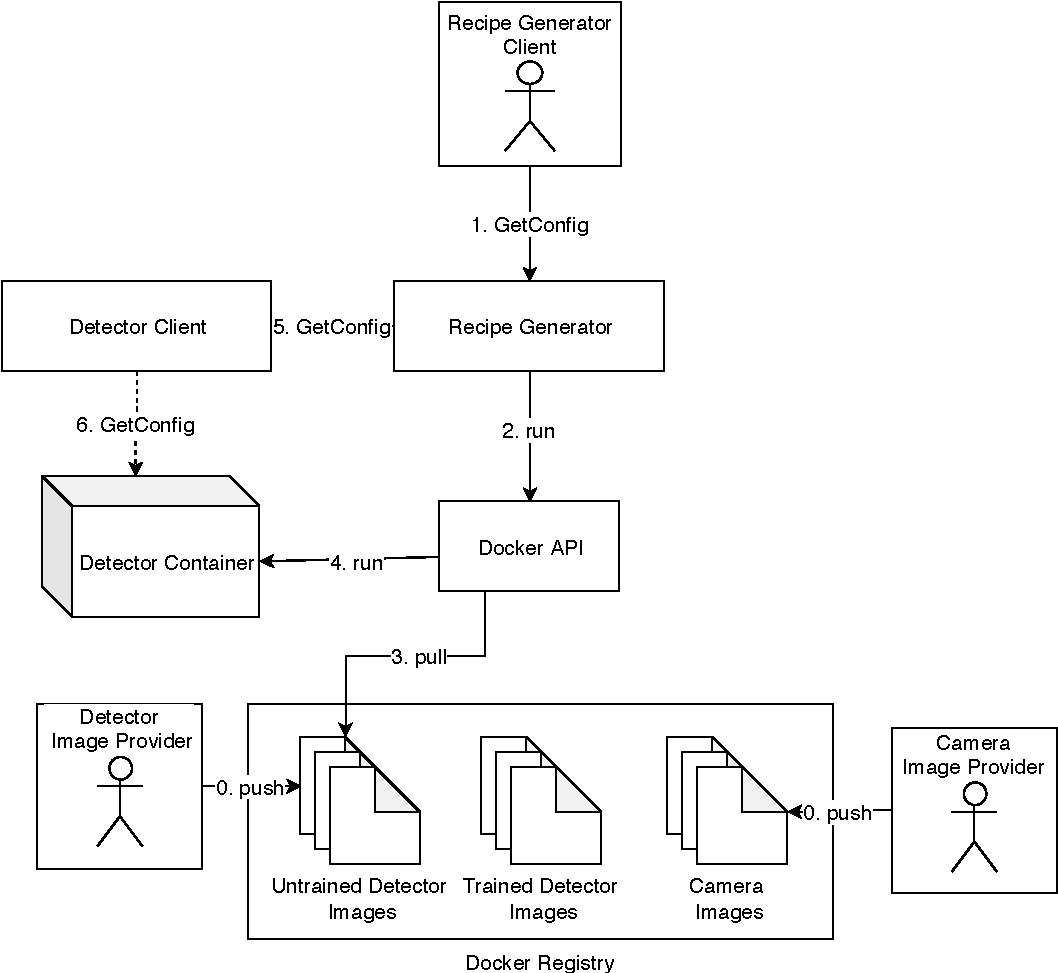
\includegraphics[width=\textwidth]{img/SequenceDiagram-GetConfig.pdf}
	\caption{Sequence Diagram - GetConfig}
	\label{fig:SequenceDiagram-GetConfig}
\end{figure}

\begin{enumerate}
    \item \mintinline{Python}{GetConfig} is called by the RG client which could be a machine operator, a PLC or a production planner. \begin{tabbing}
            space \= space \= spacespacespace \= spacespacespacespace \= spacespacespace \kill
            \>  GetConfig(\\
            \>  \>  (out)	 \> 	String           \> Config); 
        \end{tabbing} \label{sign:getconfig}
        
    \item To run this method, it is necessary to instantiate an instance of the \mintinline{Python}{DockerApi} class which connects to a Docker registry provided by environment variables. You need to provide an \mintinline{Python}{imageName} when instantiating. Running the \mintinline{Python}{run} method does not require any input, a \mintinline{Python}{port} can be stated optionally (default 8000 for detectors, 8011 for cameras): \begin{tabbing}
    space \= space \= spacespacespace \= spacespacespacespace \= spacespacespace \kill
    \>  run\_container(\\
    \>  \>  (in)	 \> 	Int          \> port\\
    \>  \>  (out)	 \> 	ContainerObject           \> container); 
    \end{tabbing}
    \mintinline{Python}{ContainerObject} will be returned by the nested method call explained in point 4. \label{sign:runcontainer}
    \item \mintinline{Python}{Pull} is invoked by the run method in point 4 and needs no call. \label{sign:pull}
    \item See~\cite{Docker-Py-Documentation2019Docker2019} for a detailed reference of \mintinline{Python}{run}: 
    \begin{tabbing}
    space \= space \= spacespacespace \= spacespacespacespace \= spacespacespace \kill
    \>  run(\\
    \>  \>  (in)	 \> 	String          \> imageName\\
    \>  \>  (in)	 \> 	boolean          \> detach\\
    \>  \>  (in)	 \> 	boolean    \> autoremove\\
    \>  \>  (in)	 \> 	Dict   \> ports\\
    \>  \>  (in)	 \> 	boolean   \> stderr\\
    \>  \>  (in)	 \> 	boolean          \> stdout\\
    \>  \>  (out)	 \> 	ContainerObject           \> container); 
    \end{tabbing}\label{sign:run}
    \item \mintinline{Python}{GetConfig} is a member of \mintinline{Python}{DetectorClient} which is initialized with a gRPC channel to the detector and interfacing stub. GetConfig can be called with no input. For the signature see~\ref{sign:getconfig}.
    \item \mintinline{Python}{GetConfig} gathers the config via gRPC. For the signature see point~\ref{sign:getconfig}.
\end{enumerate}


\subsection{Train}
See figure \ref{fig:SequenceDiagram-Train}.
\begin{enumerate}
    \item \mintinline{Python}{Train} uses a CAD file and an optional configuration file as input to train the detector for later usage. It returns the Train result and optional camera image files for result representation.
        \begin{tabbing}
        space \= space \= spacespacespace \= spacespacespacespace \= spacespacespace \kill
        \>  Train(\\
        \>  \>  (in)	 \> 	file          \> cad\\
        \>  \>  (in)	 \> 	file          \> conf\\
        \>  \>  (out)	 \> 	file          \> image\\
        \>  \>  (out)	 \> 	String           \> result); 
        \end{tabbing}\label{sign:train}
    \item See point~\ref{sign:runcontainer} in~\ref{subsec:getconfig}.
    \item See point~\ref{sign:pull} in~\ref{subsec:getconfig}.
    \item See point~\ref{sign:run} in~\ref{subsec:getconfig}.
    \item \mintinline{Python}{Train} is a member of a \mintinline{Python}{DetectorClient} which is initialized with a gRPC channel to the detector and interfacing stub. See point~\ref{sign:train} for the signature.
    \item \mintinline{Python}{Train} gathers the config via gRPC. See point~\ref{sign:train} for the signature.
    \item \mintinline{Python}{commit} creates an image of the running detector container instance and pushes it to a repository. It is a method part of the Docker Python framework described in~\cite{Docker-Py-Documentation2019Docker2019}, see a detailed description of the method there. Here, the method pushes the image to the repository defined by environment variables.
    \begin{tabbing}
    space \= space \= spacespacespace \= spacespacespacespace \= spacespacespace \kill
    \>  Train(\\
    \>  \>  (in)	 \> 	ContainerObject          \> containerinstance\\
    \>  \>  (out)	 \> 	String           \> result); 
    \end{tabbing}\label{sign:commit}
    \item \mintinline{Python}{create_image} is part of \mintinline{Python}{commit}.
    \item \mintinline{Python}{push} is part of \mintinline{Python}{commit}.
\end{enumerate}

\begin{figure}[ht]
	\centering
  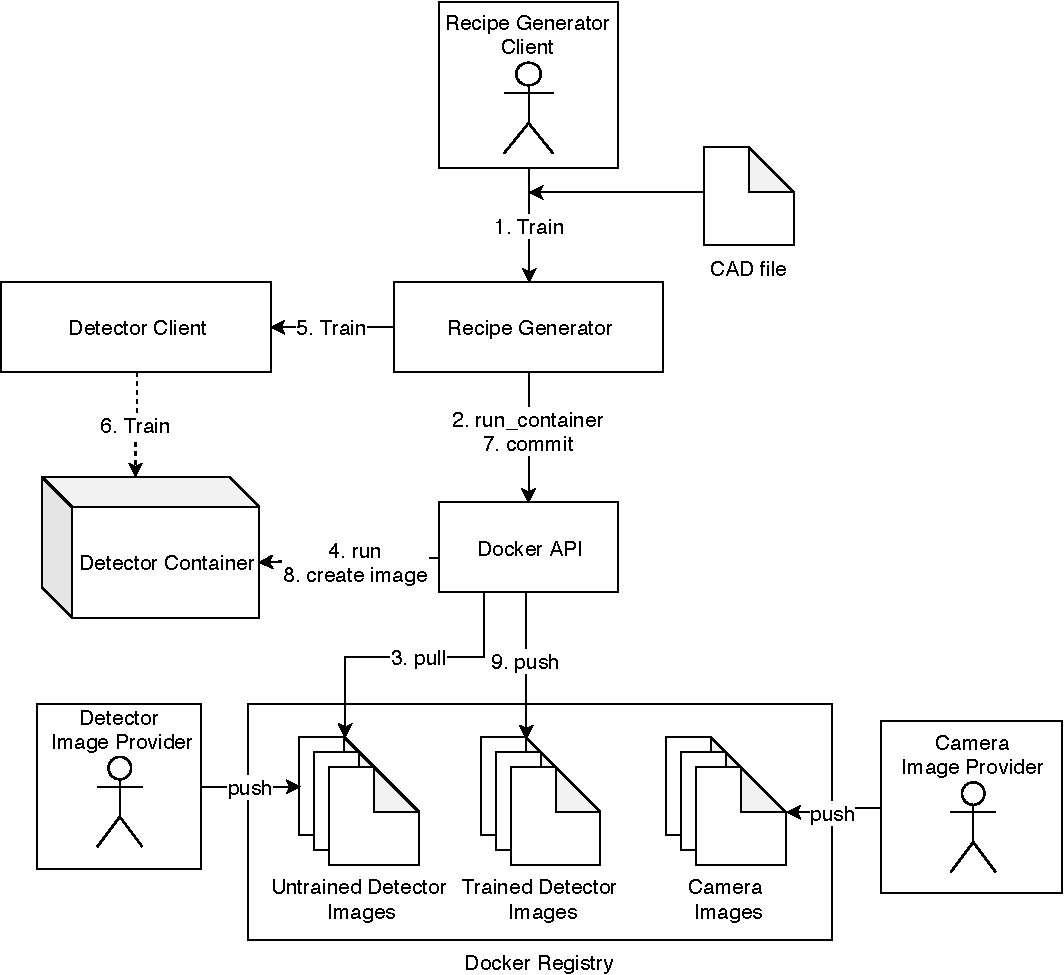
\includegraphics[width=\textwidth]{img/SequenceDiagram-Train.pdf}
	\caption{Sequence Diagram - Train}
	\label{fig:SequenceDiagram-Train}
\end{figure}

\subsection{GenRecipe} \label{subseb:genrecipe}
See figure~\ref{fig:SequenceDiagram-GenRecipe}.
\mintinline{Python}{GenRecipe} takes a docker image pair (\mintinline{Python}{i}) and saves it in the recipe storage. The pair consists of one camera and one detector docker image. As of now, the method saves the pair as a file in a folder. In the future, this could be done with a database. The filename is a generated UUID later used as \mintinline{Python}{ExternalId}.
\begin{enumerate}
    \item \mintinline{Python}{GenRecipe} initializes an instance of \mintinline{Python}{Recipe} with an \mintinline{Python}{ExternalId} and calls its \mintinline{Python}{add} method.
    \begin{tabbing}
    space \= space \= spacespacespace \= spacespacespacespace \= spacespacespace \kill
    \>  GenRecipe(\\
    \>  \>  (in)	 \> 	String          \> i\\
    \>  \>  (out)	 \> 	String          \> ExternalId); 
    \end{tabbing}
    \item \mintinline{Python}{add} takes the image pair (\mintinline{Python}{imageList}) as input and \mintinline{Python}{write}s it into recipe/recipes folder with \mintinline{Python}{ExternalId} as the filename.
    \begin{tabbing}
    space \= space \= spacespacespace \= spacespacespacespace \= spacespacespace \kill
    \>  add(\\
    \>  \>  (in)	 \> 	String          \> imageList);  
    \end{tabbing} \label{sign:add}
    \item \mintinline{Python}{write} writes \mintinline{Python}{imageList} as comma-separated String into a file. The method is part of \mintinline{Python}{add}. \label{sign:write}
\end{enumerate}

\begin{figure}[ht]
	\centering
  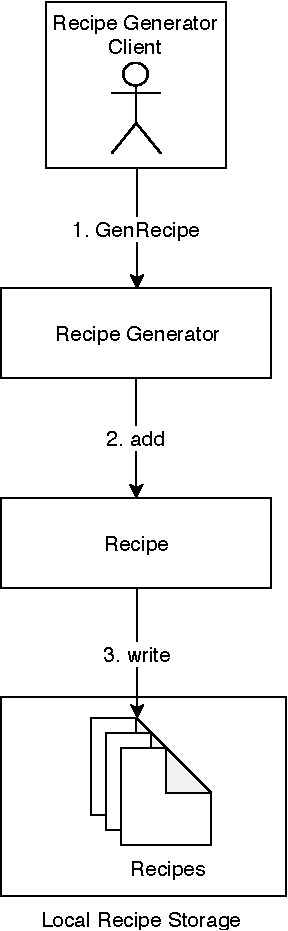
\includegraphics[height=0.5\textheight]{img/SequenceDiagram-GenRecipe.pdf}
	\caption{Sequence Diagram - GenRecipe}
	\label{fig:SequenceDiagram-GenRecipe}
\end{figure}

\subsection{Transfer}
\mintinline{Python}{Transfer} fetches the recipe and transmits it over to the OPC UA Vision server recipe management. The server has to be running for a successful method call. In the demo implementation, the recipe storage of the RG and the OPC UA Vision server are the same (see~\ref{fig:SequenceDiagram-Transfer}). A recipe is a pair of docker image names, the list being decorated with an \mintinline{Python}{ExternalId}. The OPC UA Vision client can be a PLC or a human machine operator. See figure \ref{fig:SequenceDiagram-Transfer}.

\begin{enumerate}
    \item \mintinline{Python}{Transfer} instantiates an instance of \mintinline{Python}{Recipe} with \mintinline{Python}{extid} and transfers the gathered image list via an OPC UA Client to the server.
    \begin{tabbing}
    space \= space \= spacespacespace \= spacespacespacespace \= spacespacespace \kill
    \>  Transfer(\\
    \>  \>  (in)	 \> 	String          \> extid\\
    \>  \>  (out)	 \> 	String          \> ExternalId);
    \end{tabbing} \label{sign:Transfer}
    \item See point \ref{sign:Transfer}.
    \item 
    \begin{tabbing}
    space \= space \= spacespacespace \= spacespacespacespace \= spacespacespace \kill
    \>  get\_recipe(\\
    \>  \>  (out)	 \> 	Array          \> imageList); 
    \end{tabbing}
    \item 
    \begin{tabbing}
    space \= space \= spacespacespace \= spacespacespacespace \= spacespacespace \kill
    \>  add\_recipe(\\
    \>  \>  (in)	 \> 	String          \> ExternalId\\
    \>  \>  (in)	 \> 	Array          \> imageList\\
    \>  \>  (out)	 \> 	String          \> Result); 
    \end{tabbing}\label{sign:addrecipe}
    \item OPC UA Client opens a TCP connection to OPC UA Server and then calls \mintinline{Python}{AddRecipe}. See point~\ref{sign:addrecipe} for the signature.
    \item See point~\ref{sign:add} in subsection~\ref{subseb:genrecipe}.
    \item See point~\ref{sign:write} in subsection~\ref{subseb:genrecipe}.
\end{enumerate}

\begin{figure}[ht]
	\centering
  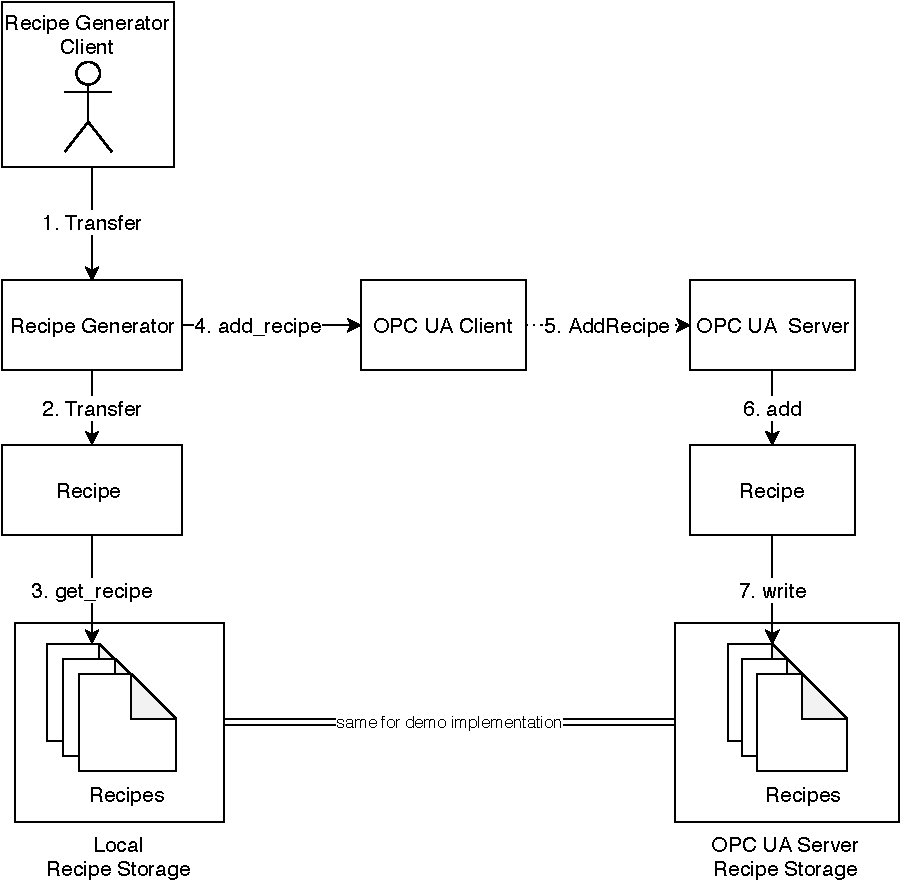
\includegraphics[width=0.7\textwidth]{img/SequenceDiagram-Transfer.pdf}
	\caption{Sequence Diagram - Transfer}
	\label{fig:SequenceDiagram-Transfer}
\end{figure}

\subsection{Prepare}
\mintinline{Python}{Prepare} runs the two docker images defined by \mintinline{Python}{ExternalId} returns. See figure~\ref{fig:SequenceDiagram-Prepare}.

\begin{enumerate}
    \item 
    \begin{tabbing}
    space \= space \= spacespacespace \= spacespacespacespace \= spacespacespace \kill
    \>  PrepareRecipe(\\
    \>  \>  (in)	 \> 	String          \> ExternalId\\
    \>  \>  (out)	 \> 	String          \> Result); 
    \end{tabbing}
    \item OPC UA Server imports the same \mintinline{Python}{Recipe} class as the RG. It instantiates an instance of the class and calls the prepare method.
    \item From here onward the process is analogous to the methods described before.
\end{enumerate}

\begin{figure}[ht]
	\centering
  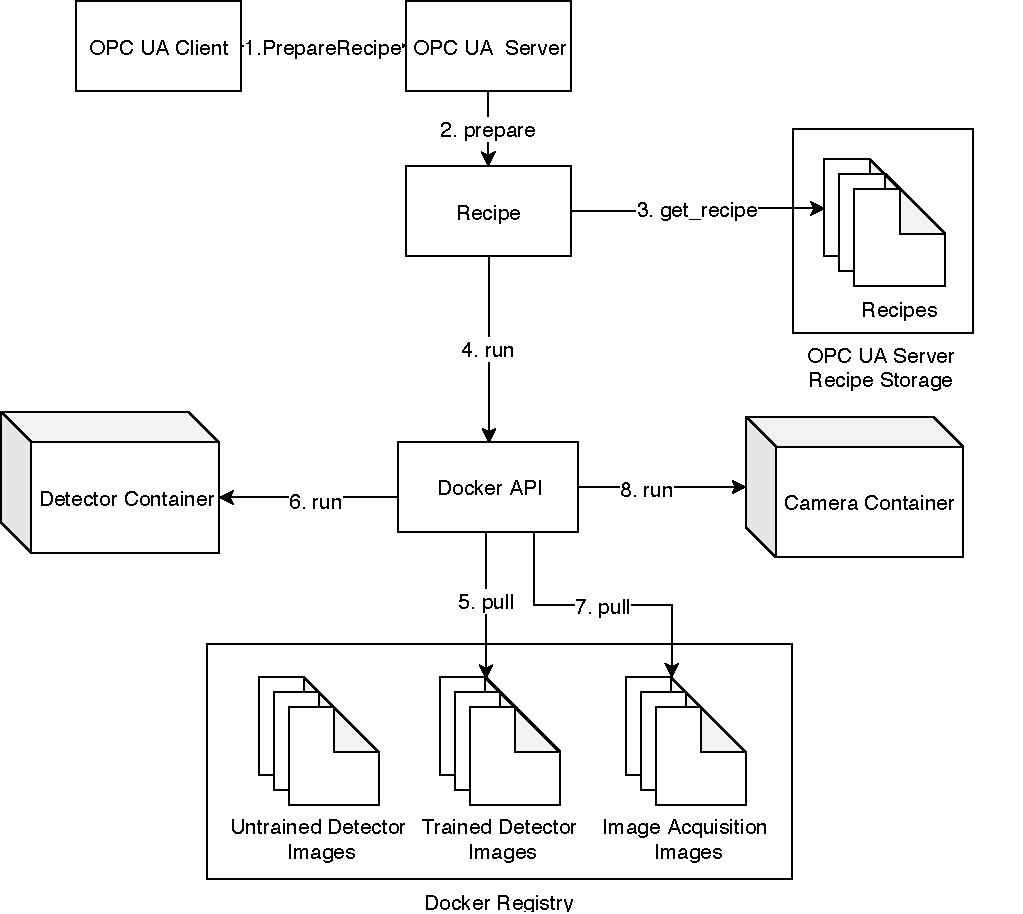
\includegraphics[width=0.7\textwidth]{img/SequenceDiagram-Prepare.pdf}
	\caption{Sequence Diagram - Prepare}
	\label{fig:SequenceDiagram-Prepare}
\end{figure}

\subsection{Test}
See figure~\ref{fig:SequenceDiagram-Test}.

\begin{enumerate}
    \item OPC UA Vision server creates a \mintinline{Python}{JobId} unique for this job and returns it along with the result.
    \begin{tabbing}
    space \= space \= spacespacespace \= spacespacespacespace \= spacespacespace \kill
    \>  StartSingleJob(\\
    \>  \>  (in)	 \> 	String          \> RecipeId\\
    \>  \>  (out)	 \> 	Dict          \> Pose \\
    \>  \>  (out)	 \> 	String          \> JobId); 
    \end{tabbing}
    \item 
    \begin{tabbing}
    space \= space \= spacespacespace \= spacespacespacespace \= spacespacespace \kill
    \>  GrabImage(\\
    \>  \>  (out)	 \> 	bytes          \> image); 
    \end{tabbing} \label{sign:grabimage}
    \item The camera client calls the camera container located on a camera or camera image storage to fetch and return a camera image. See point~\ref{sign:grabimage} for the signature.
    \item \mintinline{Python}{Test} uses the grabbed image of point~\ref{sign:grabimage} to call detector client's \mintinline{Python}{Test} method. \mintinline{Python}{Test} optionally returns images to illustrate its result. 
    \begin{tabbing}
    space \= space \= spacespacespace \= spacespacespacespace \= spacespacespace \kill
    \>  Test(\\
    \>  \>  (in)	 \> 	bytes          \> image\\
    \>  \>  (out)	 \> 	Dict          \> Pose \\
    \>  \>  (out)	 \> 	bytes          \> image \\
    \>  \>  (out)	 \> 	String          \> JobId); 
    \end{tabbing}\label{sign:Test}
    \item See point~\ref{sign:Test}.
\end{enumerate}

\begin{figure}[ht]
	\centering
  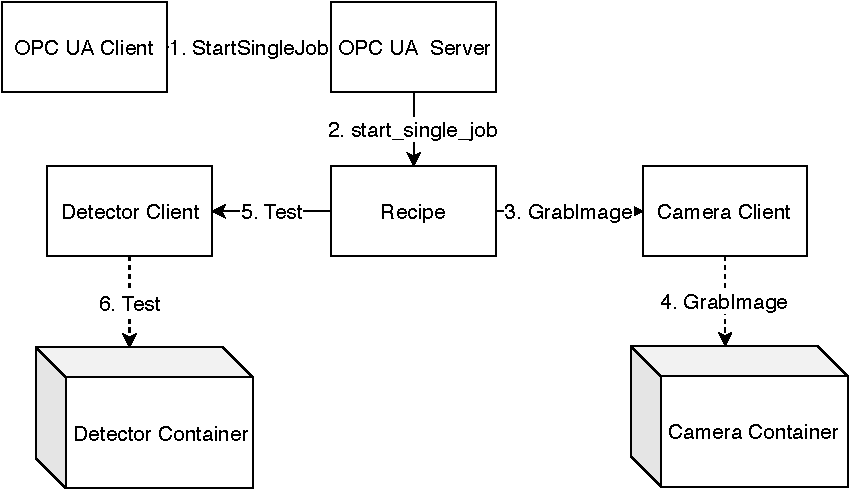
\includegraphics[width=0.7\textwidth]{img/SequenceDiagram-Test.pdf}
	\caption{Sequence Diagram - Test}
	\label{fig:SequenceDiagram-Test}
\end{figure}

\section{Software Architecture of Recipe Generator}
The architecture of RG divides into the same components as presented in the concept in figure~\ref{fig:concept}. So does the folder structure:
\begin{itemize}
    \item camera. Represents the blueprint of a gRPC interface of a camera with the \mintinline{Python}{GrabImage} method.
    \begin{itemize}
        \item images. Storage for grabbed camera images.
    \end{itemize}
    \item detector. Represents the blueprint of a gRPC interface of a detector with the \mintinline{Python}{Train} and \mintinline{Python}{Test} method.
    \item dockerapi. Handles Docker registry administration, container running and more Docker features.
    \item opc\_ua. A Python OPC UA server.
    \begin{itemize}
        \item recipes. Recipe management storage of the OPC UA server.
    \end{itemize}
    \item recipe. A template for recipies calling the standardized methods of camera and detector in sequence.
    \begin{itemize}
        \item recipes. Recipe storage of the RG.
    \end{itemize}
\end{itemize}

When using RG, only recipe\_generator.py and opc\_ua\_client.py have to be called from a command-line interface. A help is provided, callable with the help flag:

\begin{minted}{python}
    py path_to_file/recipe_generator.py --help
\end{minted}

The source code is provided with comments and docstrings where necessary. All Python modules have no GUI, instead, they are command line based. However, the use of, e.g., UA Expert for calling OPC UA Vision methods is possible. 

See figures~\ref{fig:Classes} and~\ref{fig:Packages} for an illustration of the used classes and packages in the demo implementation. The UML diagrams were generated automatically with Pyreverse by scanning the source code~\cite{Anclin2008Pyreverse2019}.

The classes ending with Servicer and Stub are generated by gRPC. gRPC server classes need to inherit the Servicer class (e.g., Detector inherits DetectorServicer). In case the proto files are enhanced or new files are created, new Servicer and Stubs can be created with a build command similar to:

\begin{minted}{python}
    py -m grpc_tools.protoc  -I. --python_out =. //
        --grpc_python_out =. .\ camera.proto
\end{minted}

Note that the command must be executed from the directory of the respective proto file. 

Recipe class is responsible for recipe administration and calling. For example, \mintinline{Python}{prepare()} runs the detector and camera container of the recipe instance.
\begin{figure}[ht]
	\centering
  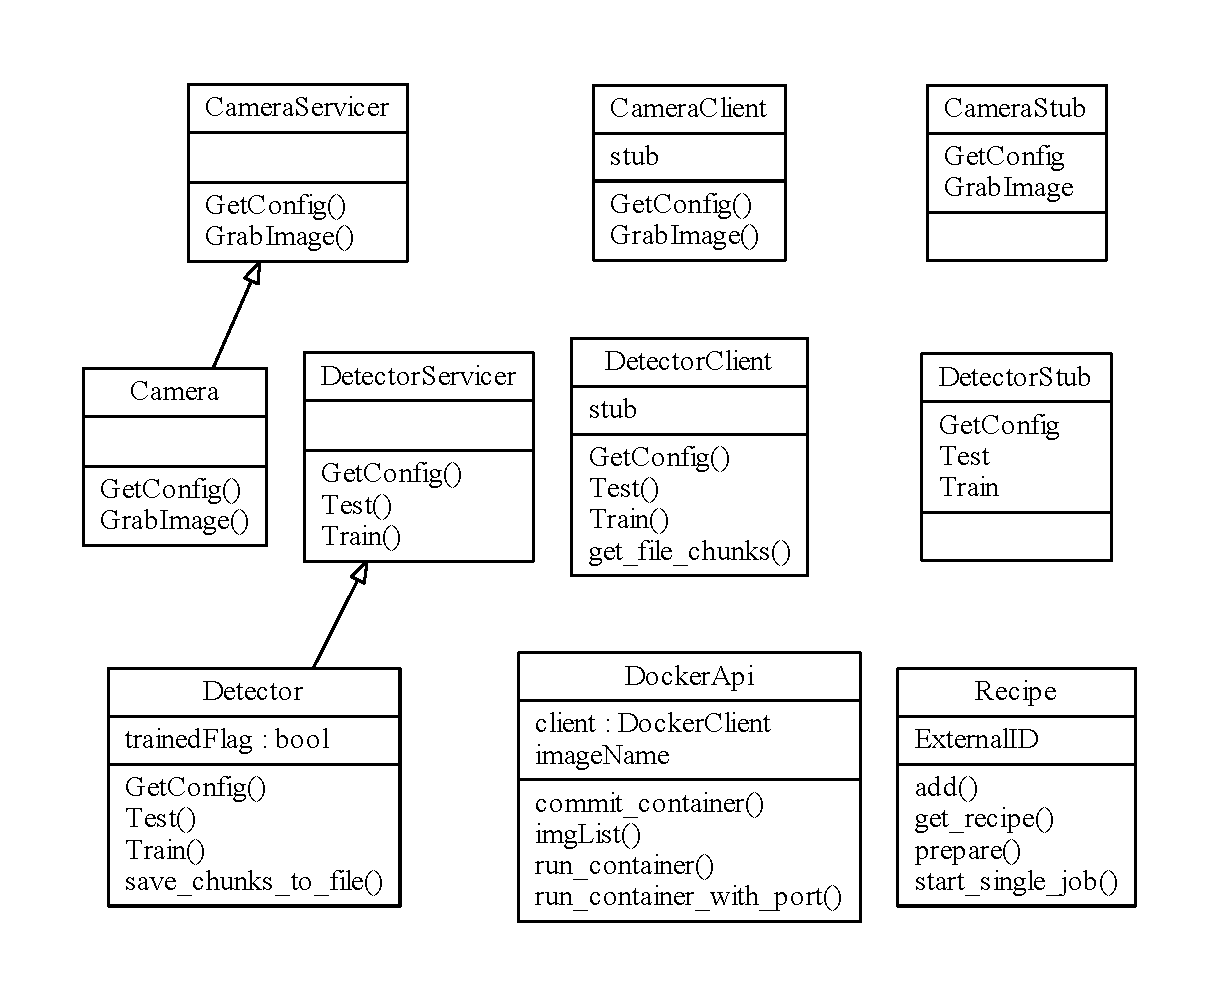
\includegraphics[width=0.9\textwidth]{img/classes.pdf}
	\caption[Class diagram]{Class diagram. Arrows denote inheritance.}
	\label{fig:Classes}
\end{figure}

The package diagram gives an overview of the dependency complexity of the different components. Through the cohesion of the components, methods can be reused effectively and in a way that is following the RG concept. An example is the Docker API (dockerapi.dockerapi) that is used by the RG (recipe.recipe\_generator) and the recipe (recipe.recipe).
\begin{figure}[ht]
	\centering
  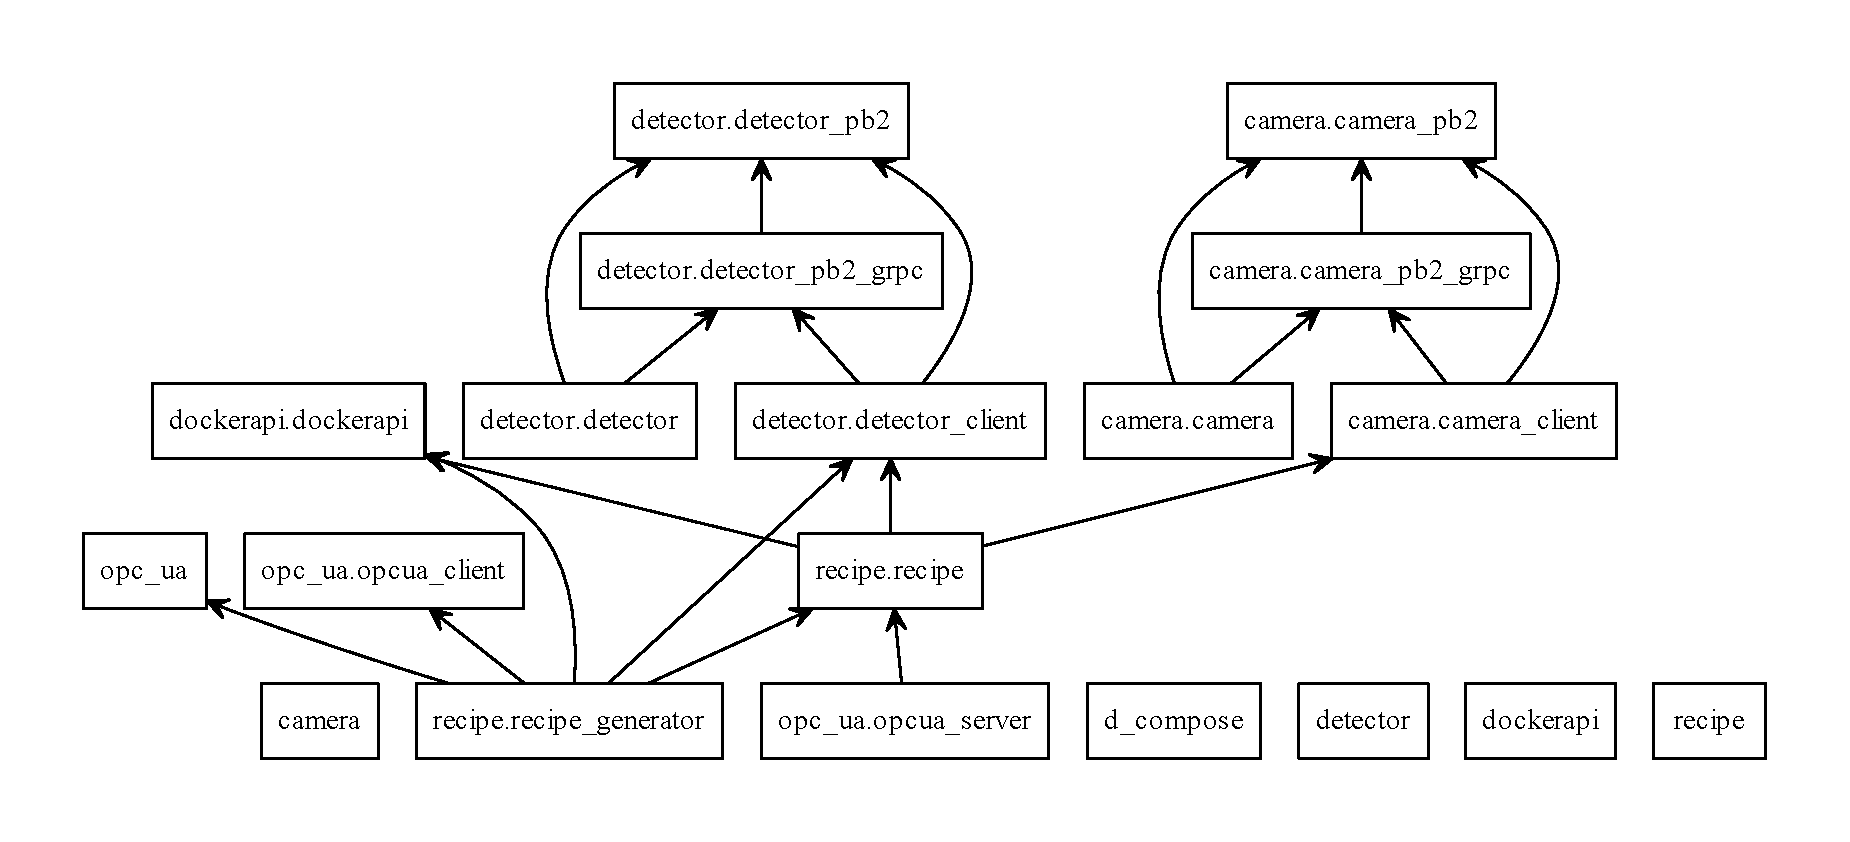
\includegraphics[width=\textwidth]{img/packages.pdf}
	\caption[Package diagram]{Package diagram. Arrows denote imports.}
	\label{fig:Packages}
\end{figure}

\section{Virtualization Technology: Docker}
\subsection{Pro}
Realizing a SOA calls for means of decoupling the components and efficient tooling. Docker is the technology which was used here due to the following reasons:
\subsubsection{Dependencies of Components are handled smoothly} 
Every docker image can pull the packages and system variables it needs as specified in the dockerfile. For example, one detector may depend on openCV 2.7.1 while another detector depends on 1.8. Both docker images that are built using their respective dockerfile are independent of each other. If no virtualization technology was used here, a dependency handling for the whole recipe management would be necessary. In the case of two openCV versions, just a slight modification of the framework may be necessary. A more drastic example would be detectors that rely on different .NET frameworks which might not be able to coexist on a system.
\subsubsection{Platform Independency}
 Platform in this context refers to the operating system, e.g. Windows or Linux. The independency is twofold. Firstly, the docker engine runs on Linux (CentOS, Debian, Fedora, Oracle Linux, RHEL, SUSE and Ubuntu) and Windows Server. In an industrial context, both platforms are present and should be supported for maximum flexibility.
\subsubsection{Orchestration}
 Containers can be scaled if more resources are needed, monitoring and load balancing are possible and the network over which the containers communicate can be configured. See e.g. Mandy Waite's contribution to DevFest Ukraine in 2015 for more information.~\cite{Waite2015ScalableContainers}
\subsubsection{Docker Hub}
 Docker offers (semi)-public or private repositories. They can be used by detector or camera providers to push their docker images and for the recipe management to pull them. As base image, there are preconfigured environments available. For this implementation, a fully functioning Python environment was used as base Docker image. To prevent know-how-leaking of ODMs, the accessibility to the images on the hub can be restricted. In this implementation, a local repository was used with full accessibility to the Docker images.
 \subsubsection{Calculations on Graphical Processing Unit}
 Some detectors need excessive calculation power. If applicable, the graphical processing unit of the bare metal server the docker engine is running on can be added. It should be kept in mind that with this technique the detector docker image is dependent not only on the docker engine but also on the bare metal hardware. Thus, this option should be used with caution and only if needed.
\subsection{Contra}
\subsubsection{Lock-in}
The reason against using Docker is making all involved parties introduced in appendix~\ref{sec:involvedparties} use docker. Camera and detector docker image providers need to add a dockerfile for building the image and pushing it to the repository. On the recipe management-side a docker engine compatible infrastructure has to be provided. 

\section{Detector and Camera Communication: gRPC}
To implement the Train, Test, GetConfig and GrabImage methods defined in~\ref{detectormethods} gRPC was used. In the current implementation, the TCP ports on which the detector and camera server listen is static. Detectors listen on port 8000, cameras on port 8011. The approach of gRPC service interfaces comes with certain pros and cons:
\subsection{Pro}
\subsubsection{Simple Service Definition}
In proto files, the service RPCs and input/output types are defined. With protoc, the protocol buffer compiler, it is possible to generate place holders for clients and servers, called stubs. These place holders are the base for every camera or detector docker image provider. For a complete overview of the created proto files see~\ref{proto}. 
\subsubsection{Multilingual}
Idiomatic stubs can be generated in 12 languages~\cite{gRPC-Documentation2019Last2019}. This is a great advantage for every provider since no wrapping or complete rewriting of code in a possibly unknown language has to be done.
\subsubsection{Backward Compatibility}
According to Sam Newman, it is crucial to be able to deploy new servers without having to deploy clients at the time or otherwise dependently~(\cite{Newman2015BuildingMicroservices}, page~79). This is easily done with gRPC and proto3 syntax - as long as no fields are deleted or the numbers change, older clients will still be able to work with new servers.
\subsubsection{REST Gateway}
gRPC's ecosystem offers a protobuf/JSON gateway as described in detail in section~\ref{sec:grpc}. In the current implementation, this is not done. Note that as of today, it is not supported to send files as streams via the gateway. As a workaround, files can be converted into base64 encoded strings. 
\subsubsection{Streaming}
gRPC supports HTTP/2. Especially for large files this is an advantage because multiplexed, bi-directional streams are supported. This allows for high-performance file transfer. In this implementation, a byte stream was used for the Train method of the detector. See~\ref{proto} for the proto file and~\ref{sec:grpcpython} for an example python implementation.

\subsection{Contra}
\subsubsection{Lock-in}
As well as for Docker as virtualization technology gRPC might mean extra work for detector and camera providers. Although stubs can be provided, developers still need to adhere to the service definition in the proto file.

\subsubsection{Networks will fail}
According to Sam Newman, networks can never be trusted~(\cite{Newman2015BuildingMicroservices}, page~76). So, appropriate fail mechanisms have to be provided. For example, a buffering of messages is possible in case of a corrupt gRPC channel. This is not implemented in the demo framework yet.

\section{Object Detection Methods used}
As for the demo framework implementation, only dummy detection methods were used. There is no ODM behind the Train and Test methods, just a simple snippet receiving, saving and returning data. For the config file, an arbitrary string with no further use was sent between services; for the camera image and CAD files, a JPG demo camera image was sent. The relevant sections in source code are marked with comments so the framework architect and Docker image providers know where to include their code snippets.

\section{Differences to OPC UA Vision Specification}
There are major simplifications made of the OPC UA Vision specification. This is mostly due to the fact that there was no \textbf{XML nodeset} released by the time of implementation. The nodeset would have allowed to import the entire information model to an OPC UA server. Instead I had to create the methods and necessary data types manually.

\textbf{Recipe transfer} has been simplified since the OPC UA Vision server and the RG share their recipe storage and Docker registry, it is sufficient to transfer the ExternalId with no additional content required. This might not be the case in a productive environment, where the topology does not allow sharing the same storage and registry. If they share at least the Docker registry, then it is possible to reprogram the ExternalId to a string of concatenated Docker image names, e.g. detector:latest-camera:latest. If they share none of the two, then additional image content transfer via OPC UA has to be done or the OPC UA Vision server Docker registry needs to be managed externally.

According to the OPC UA Vision specification, StartSingleJob is an asynchronous method which triggers recipe execution and the state machine to transit from Ready to SingleExecution (see figures~\ref{fig:OPCStateMachineAutomatic} for a sequence diagram of the automatic mode of the state machine and~\ref{fig:runtimeviewexec} for a sequence diagram of recipe execution). The entire \textbf{state machine} of the OPC UA Vision server was neglected due to the time restrictions of the thesis. As a workaround, all methods were implemented synchronously. In consequence, the event containing the detection result is not sent but instead the pose is directly returned by StartSingleJob.



    \chapter{Fazit und Ausblick\label{cha:chapter6}}




    \chapter{Conclusion\label{cha:chapter7}}

In this thesis, I tried to generate ODS with varying detection methods and interfaces automatically. The title divides into three challenges:
\begin{itemize}
    \item Generating ODS automatically
    \item Handling ODS with varying detection methods
    \item Handling ODS with varying interfaces
\end{itemize}
In response, I created a SOA concept which tackles these challenges. Generating ODS automatically has been undergird with a supporting framework. It helps to combine the necessary components of camera image acquisition, ODMs and returning the pose in a standardized way. These services must adhere to a versioned semantic Train and Test definition, which is generic enough to comprehend a broad set of ODMs. Expanding the semantic to a new version is of little effort.\\
The service interfaces are currently limited to gRPC or REST. Albeit this covers two established interfaces, they lack certain functionality such as message queuing. A more holistic implementation is desirable for the future, e.g. with an ESB. This would allow for even greater interoperability and reliability.

Further works include fulfilling all OPC UA Vision specification aspects once they are fully released. Especially the drill down to component level and a specification of how to interface e.g. cameras will bring about the possibility for high-speed implementation of new components.

% ---------------------------------------------------------------
%\backmatter % no page numbering from here
		
		% if you want to provide a glossary with explanations of important terms put it in here

    \bibliographystyle{vancouver}
    \bibliography{./bib/references}
    
    
\appendix
% \begin{appendices}

\chapter{Roles}
\label{sec:involvedparties}
\pagenumbering{roman}
\extrarowsep=0.6cm\begin{longtabu} to \linewidth{lX}
    Recipe Generator Client & The instance calling recipe generator methods Train, Test, Transfer, GenRecipe and GetConfig. It needs to have a certain intelligence to decide when to call which methods with the appropriate parameters. In the current state, this will most likely be a production engineer. It is assumed that adding or altering a recipe does not happen very frequently. In later use where more business intelligence resides inside recipe generator, the client could be a component, e.g. a PLC.\\ 
    Detector Image Provider & The instance developing new ODMs. This could be research teams, community projects like OpenCV or OD specialists of the company using recipe generator. For every new ODM, it is necessary to adhere to the recipe generator API or, for a new pattern of ODMs, update the recipe generator API.\\
    Camera Image Provider &  	The instance providing new camera hardware and capable software of interacting with recipe generator.\\ 
    Framework Architect & The author or contributor of recipe generator. He or she is responsible for the SOA design, continuous development and integration and updated proto files. Often the same person as the recipe genetor client.
\end{longtabu}


\chapter{Example of a Recipe Life Cycle}
\label{chap:recipelifecycle}
To illustrate recipe management, here is a possible life cycle of a recipe taken from the OPC UA Vision specification appendix~\cite{VDMA2018OPC40100-1:2018-11}. Note that the method signatures are not necessarily exact here. 
\begin{enumerate}
    \item A recipe for ProductId-m is created externally (often centrally). 
    \item The recipe is pushed to the vision system with ExternalId-1, ProductId-m (using AddRecipe())
    \begin{itemize}
        \item It is stored there with ExternalId-1, InternalId-11.
        \item It is linked to ProductId-m on the vision system
    \end{itemize}
    \item There are further possible actions on the recipe without any particular order.
    \begin{itemize}
        \item The recipe may be edited locally later, keeping its ExternalId-1 and receiving InternalId-12.
        \item A (binary) different version of the recipe with the same ExternalId-1 may be pushed to the vision system later, receiving InternalId-13.
        \item The recipe may be linked later to ProductId-n on the vision system. Note that the external recipe 
        management does not concern itself with the InternalIds of the recipes on different vision systems. If 
        there are, due to one of these operations, several recipes on the vision system with identical 
        ExternalIds but different InternalIds, the vision system/server combination has no means of telling 
        which of these was targeted by the environment. It may choose to link all of them, or the newest one, 
        or the latest one pushed (ignoring internally edited ones). This is outside the scope of this specification.
    \end{itemize}
    \item The automation system is undergoing a change-over process to a specific product, namely ProductId-m. It 
    will re-tool the vision system
    \begin{itemize}
    \item by calling PrepareRecipe(ExternalId-1); the vision system then selects one of the existing recipes with 
    ExternalId-1 based on internal rules.
    \item by calling PrepareRecipe(ProductId-m); the vision system then selects one of the existing recipes 
    linked to ProductId-m based on internal rules. 
    \end{itemize}
    \item The vision system is commanded to process a specific product
    \begin{itemize}
        \item by calling StartJob(ExternalId-1); the vision system then starts processing with the recipe prepared for ExternalId-1. 
        \item by calling StartJob(ProductId-m); the vision system then starts processing with the recipe prepared for ProductId-m. 
        \item by calling StartJob(ExternalId-2); the vision system then throws an error because no such recipe has 
        been added or prepared.
        \item by calling StartJob(ProductId-p); the vision system then throws an error because no such recipe has 
        been added or prepared. 
    \end{itemize}
    \item If there is no error, the vision system carries out its task, going through the Executing state to return to state Ready waiting for further instructions. There are many other possibilities of errors, e.g. trying to prepare a recipe which is actually a sub-recipe, i.e., not capable of being processed by itself. 
\end{enumerate}

% \chapter{OPC UA Vision Method Signatures used in this Thesis}

\chapter{Proto Files}
\label{proto}
\section{Detector}
\lstinputlisting[language=protobuf3,style=protobuf]{img/detector.proto}

\section{Camera}
\lstinputlisting[language=protobuf3,style=protobuf]{img/camera.proto}

\endinput
% \end{appendices}


\end{document}
